% Confinement scaling as a linear algebra problem
%
% Build:  tectonic paper/paper.tex        (or: pdflatex paper/paper.tex, twice)
%
% Submission notes:
%   * \date is deliberately a fixed date, not \today. A DOI record and an arXiv
%     posting are permanent, and a paper whose date is "whenever this happened
%     to compile" disagrees with itself between the archived PDF and any later
%     rebuild. Bump it when the content changes, not when the file is touched.
%   * Figures resolve through \graphicspath, so this source builds both in the
%     repository (../results/) and from the flat directory arXiv unpacks into.
%     Assemble that flat submission with `make arxiv`.
\documentclass[12pt,a4paper]{article}

\usepackage[margin=2.4cm]{geometry}
\usepackage[T1]{fontenc}
\usepackage{lmodern}
\usepackage{amsmath}
\usepackage{booktabs}
\usepackage{graphicx}
% Repository layout first, then the flat layout `make arxiv` produces.
\graphicspath{{../results/}{./}}
% Figures are named without an extension so the vector copy wins where there
% is one. IOP asks for vector line art in preference to raster, and the PDF
% of these axes is the smaller file as well.
\DeclareGraphicsExtensions{.pdf,.png}
\usepackage{caption}
\usepackage{microtype}
\usepackage[hidelinks]{hyperref}
\usepackage{xcolor}
\usepackage{siunitx}
\usepackage[section]{placeins}
% Referees ask for line numbers and some submission forms do too. It is not on
% by default because this source produces one PDF, and that PDF is also the one
% the DOI archives and arXiv posts, where numbered lines are wrong. Uncomment
% for a review upload and rebuild; do not commit the result.
% \usepackage[mathlines]{lineno}\linenumbers

\captionsetup{font=small,labelfont=bf}
\setlength{\parskip}{0pt}
\sisetup{detect-all}
% Long \texttt{} identifiers (scikit-learn class names) are single unbreakable
% words wider than the slack a 12 pt line normally carries. Rather than
% hyphenating a code identifier, which would be wrong to copy out, let TeX
% distribute the shortfall across the paragraph.
\setlength{\emergencystretch}{3em}

\title{\vspace{-1.4cm}\textbf{Validation protocol reverses machine-learning
model\\ rankings in tokamak energy-confinement scaling}}
\author{Liam Salcedo\thanks{Independent researcher, Montclair, New Jersey, USA.
\texttt{liamsalcedo100@gmail.com}.
ORCID: \href{https://orcid.org/0009-0001-5039-8147}{\texttt{0009-0001-5039-8147}}.}}
\date{8 September 2026}

\begin{document}
\maketitle

\begin{center}\small
Code, results, and reproducibility materials:
\url{https://github.com/lsalcedo100/FusionFlux}\\
Archived at \href{https://doi.org/10.5281/zenodo.22699744}{doi:10.5281/zenodo.22699744}
(v0.4.10; the DOI for all versions is
\href{https://doi.org/10.5281/zenodo.22215142}{10.5281/zenodo.22215142})
\end{center}

\begin{abstract}
\noindent
On the ITPA Global H-mode Confinement Database (HDB5, STD5; 6228 slices, 18 labels),
under cross-validation grouped by discharge, a random forest cuts log error by
29\% against a power law refitted in the same folds and 36\% against published
IPB98(y,2). Held out one device at a time the ordering reverses, so selecting a
confinement model on its cross-validated score does not merely fail to inform
about extrapolation: over the three models compared here it picks the worst
extrapolator. Two controls bound that. Regressing the stored energy, which moves
only the identity $\tau=W/P$ and leaves the loss power among the features,
leaves the forest worse on \textbf{9 of 13} labels and 9 of 11 devices at a mean
gap of $+0.220$; in dimensionless coordinates, where no feature is a device
label but each is built from the target, it is 11 of 13 and 9 of 11. On the
confinement time and the engineering features it is 13 of 13 and 11 of 11. The
forest's error tracks the held-out label's Mahalanobis distance from the
training at $\rho=+0.85$, against $-0.06$ for the power law. At a cut
reproducing ITER's $1.82\times$ jump in major radius the trees land nearer a
constant predictor than the power law, and 90\% split-conformal intervals fall
to 3\% and 0\% coverage at unchanged width. Two repairs help, both supplying
long-range structure rather than capacity: Connor--Taylor constraints, whose
Kadomtsev rung is free in sample, and a Gaussian process with a linear kernel
component, this work's best cross-validated model, which does not reverse.
Holding nonlinear capacity fixed and varying only the long-range mean isolates
the mechanism: the failure tracks saturation rather than flexibility.
\end{abstract}

\begin{center}\small
\textbf{Keywords:} tokamak energy confinement; confinement scaling; machine
learning; extrapolation; cross-validation; dimensional similarity; uncertainty
quantification; ITER
\end{center}

\section{Introduction}
\label{sec:intro}

A tokamak ignites when the alpha heating from its own fusion reactions covers
everything the plasma loses. The energy confinement time $\tau_E$ sets that
loss rate, which makes it a principal input to how large a next-step device has
to be. Empirical scaling remains a principal tool for projecting it to a device
that does not exist yet~\cite{ipb98}: a power law in the engineering
parameters,
\begin{equation}
\tau_E = C\, I_p^{a_1} B_t^{a_2} \bar{n}_e^{a_3} P^{a_4} R^{a_5}
         \epsilon^{a_6} \kappa^{a_7} M^{a_8},
\label{eq:powerlaw}
\end{equation}
fitted by least squares across discharges from the multi-machine confinement
database. In log space Eq.~\eqref{eq:powerlaw} is exactly a linear model, so
fitting one is ordinary least squares on a log design matrix. The reference fit
is IPB98(y,2)~\cite{ipb98}, a regression over the ITPA multi-machine database
whose exponents were used to size ITER; that database is still maintained and
republished~\cite{hdb5}, and the confinement and transport basis was revised in
2007 with IPB98(y,2) retained as the reference H-mode scaling~\cite{doyle07}.

What such a law is used for is an extrapolation, and a large one. ITER's major
radius is 1.82 times the largest machine in the database, and
SPARC~\cite{creely} is designed for a toroidal field 2.1 times the largest
recorded in it. The law is asked for a number at a point no row occupies, and
that is the regime in which a fitted regression carries no guarantee at all.

Empirical scaling is not the only route to that number. First-principles and
reduced transport models project confinement from the turbulence that sets it
rather than from a regression over machines already built, and the integrated
modelling assembled around them is a standard part of how a next-step device's
performance is now estimated~\cite{doyle07}. The machine learning in that branch
is aimed at a different target: neural surrogates are trained to reproduce a
physics-based transport model fast enough to run inside a
simulation~\cite{citrin,meneghini}, so what is being regressed is a solver
rather than a database of machines, and SPARC's core performance is projected
that way~\cite{sparccore} alongside the empirical route. Nothing below is a
claim about that branch or evidence against it. The empirical law is still
fitted, still published, still quoted as a design point and still used to
benchmark the physics-based projections, and it is the practice that selects
among empirical models that turns out not to measure what it is used for.

This paper reports two things about that regime, and both are worth separating
from the expectation that accuracy simply degrades outside the data. The first
is that the \emph{ranking} of candidate models reverses. Under cross-validation
grouped by discharge a random forest beats a power law refitted in the same
folds by 29\%; held out one whole device at a time, it is worse than that same
power law on every device scored. A practitioner following the conventional
procedure does not merely get an optimistic score for the right model, they get
the wrong model. The second is what the calibrated intervals do
\emph{instead of} widening. Split-conformal intervals set to 90\% cover 3\% and
0\% of held-out rows at a size cut matched to ITER's, and their width moves by
under 1.5\% between the two arms. The stability of the width is not itself a
discovery: a split-conformal half-width is a rank statistic of the calibration
residuals and cannot depend on the test distribution at all. The consequence is
what is being reported. A design study handed such an interval cannot tell from
the interval that it has failed, because the one quantity that would carry the
warning is fixed by the construction rather than by the data it is applied to.
Degradation is a matter of degree and can be absorbed by a margin. Neither of
these can.

A third observation follows from the same table and points at what to do about
it. On a held-out label the published IPB98(y,2) law scores 0.188 against 0.214
for the power law refitted here on the same rows and features, and 0.194 against
0.278 at the size cut. Counted the way every other comparison in this paper is
counted, it wins \textbf{9 of the 13} labels outright, at an exact
$p=0.27$ that establishes nothing on its own and a direction that is
nonetheless the same one the means give. A law fitted in 1998 to a predecessor
database transfers better than an unconstrained refit of the same functional
form on more data. Which rows each saw is part of that and is not all of it.
IPB98(y,2) was fitted under an enforced high-$\beta$ Kadomtsev constraint with
the field exponent held at 0.15~\cite{ipb98,hdb5}, which is the long-range
structure Sec.~\ref{sec:dimensional} finds to be worth having; that section
reports how much of the gap the same constraints recover on a refit here, by
rung, and where the newer published laws sit on the same surfaces, which is not
where their scores would predict.

Replacing Eq.~\eqref{eq:powerlaw} with a flexible regressor is an obvious move,
and the practice is not new: Allen and Bishop~\cite{allen} fitted a neural
network to confinement data in 1992 and reported that it beat linear regression
on an in-distribution score, which is the comparison this paper is about, made
thirty-four years ago. Machine learning has been productive elsewhere in this
field since: disruption prediction~\cite{katesharbeck}, predictors trained and
compared across two devices rather than one~\cite{rea}, transfer of a disruption
predictor to a device that supplied almost none of its training
data~\cite{zhu}, and real-time magnetic control~\cite{degrave}. The disruption
branch reached the cross-machine question first, and reached it with a target
that can be scored shot by shot on the new machine, which is what a confinement
scaling law for a device that does not yet exist cannot have. Confinement
scaling itself has been revisited with symbolic regression, which abandons the
power-law form rather than fitting it~\cite{murari}, and with a neural residual
learned on top of a frozen power law~\cite{wang}. Measured conventionally the
flexible models win. On the rows used here the random forest scores 0.128 in
log-RMSE against 0.181 for a power law refitted inside the same folds on the
same rows and features, a margin of 29\%, and against 0.199 for the published
IPB98(y,2) law, a margin of 36\%.

The two comparators are not interchangeable and both are quoted throughout.
IPB98(y,2) is a historical reference: it was derived in 1998 from version 2.8
of this database's predecessor (DB2.8) rather than from the DB5.2.3 revision
analysed here~\cite{hdb5}. That predecessor overlaps the present database
substantially in devices and operating regimes, so for most folds below the
machine being held out contributed to the data IPB98(y,2)'s exponents were
fitted on, and no claim here treats it as a fold-specific comparator fitted
without the held-out rows. The power law refitted inside each fold is the
like-for-like baseline, and the reversal below is stated against it. Every
number in this paper is scored on the nine engineering features; the
ten-column matrix of Sec.~\ref{sec:rank}, which adds IPB98(y,2)'s own
prediction to them, is reported there as a control and nowhere else. Because the
result is a negative one about a common practice, every number and figure here
regenerates from the published OSF deposit at the single commit named in Data
availability, which also gives the pinning and the test binding that hold the
prose to the generated files.

\paragraph{Related work on this database.} Four recent studies apply machine
learning to the same ITPA data and are the closest prior work. Nam and
Seo~\cite{namseo} take cross-machine transfer as their subject: they align
features to correct the covariate shift between devices and use deep ensembles
for uncertainty, validating on conditions the model has not seen, including
JET-ILW and ITER. Gao \emph{et al.}~\cite{gao} apply variational and
sampling-based Bayesian neural networks to STD5 together with individual JET,
DIII-D and ASDEX Upgrade data, reporting improved accuracy alongside posterior
uncertainty. Xiong \emph{et al.}~\cite{xiong} tune random forests and two
neural architectures by Bayesian optimisation on STD5 and report $R^{2}$ up to
0.990, with a feature-importance analysis separating spherical from
conventional tokamaks. Wang \emph{et al.}~\cite{wang} anchor a
Kolmogorov--Arnold network on a frozen power law and learn only the residual,
on this same DB5.2.3 revision. Their unanchored network interpolates accurately
and, in their words, behaves unpredictably outside the training distribution,
while anchoring it to a power-law trend substantially improves its stability
across held-out cohorts defined by parameter ranges. They also try a
Mahalanobis-distance gate at prediction time and report that it helps in some
shifted regions, is not universally beneficial, and cannot compensate for
missing device coverage.

That last work fixes what is and is not new here. A flexible model that wins the
interpolation comparison and degrades badly out of distribution, repaired by
supplying a power-law trend it cannot invent for itself, is what Wang \emph{et
al.} report on this database before this paper. What separates this work from
theirs is the unit that is held out.
Their cohorts are defined by thresholds on parameter ranges, which is
a shift constructed inside the population of machines the model has already
seen; the deployment claim a scaling law makes is about a machine that is not in
that population at all, and they say explicitly that device coverage is what
their gate cannot substitute for. Nam and Seo~\cite{namseo} likewise validate on
unseen conditions and report that cross-machine transfer is harder.
Butt \emph{et al.}~\cite{butt} do hold out whole machines on this same DB5.2.3
standard set, refitting a fixed power-law form on the machines admissible below
each target in a chosen ordering, with extrapolation as the explicit design
criterion. They score no flexible model, so no ranking between model families is
at stake there. So the
contribution is neither the first report of a reversal nor the first
machine-level holdout on this database. It is that the reversal is
measured with the device as the held-out unit, on every device the database can
score; that the ranking inverts rather than narrowing; that the calibrated
interval is measured at the same time and fails without any signal in its width;
and that flexibility and long-range saturation are separated, which says which
property to avoid rather than which model. None of these works is the target of
a criticism here; what any of them reports is what its split measures, and no
better predictor is proposed here.

Why the conventional comparison cannot settle it is a fact about the data rather
than about the models. Cross-validation on this database holds out
\emph{discharges}, and every machine in a held-out fold also appears in the
training fold, so a held-out row has hundreds of near neighbours recorded on
the same device at nearby settings. What the score quantifies is how much of
JET is predictable from the rest of JET. That a validation split should match
the generalisation being claimed, and that grouped observations flatter a model
when it does not, is well understood in fields whose data arrives in
clusters~\cite{roberts}. Inside this field, Abbate \emph{et al.}~\cite{abbate}
make the same argument for transport models rather than scaling laws: that a
model has to be scored on a large database against a baseline chosen for the use
it is put to, and that on that footing two integrated codes show no significant
advantage over a two-parameter empirical baseline for temperature profiles.
Materials informatics reached the same design from the same motive and is the
closer methodological precedent: leave-one-cluster-out cross-validation was
adopted there specifically to measure extrapolation to unseen chemistries
rather than interpolation within seen ones~\cite{meredig}, and reporting how far
a target sits from the training distribution is the applicability-domain
question that field has treated as standard for two decades~\cite{sutton}.
Neither the split nor the distance diagnostic used below is new outside fusion;
what is new is what they measure on this database.

This paper measures what the deployment-matched split costs. What is held out is
escalated in three steps, a discharge, then a database label, then a physical
device, and the same models are scored under each; a fourth comparison holds out
an entire size range, and because its held-out side is 96\% one physical machine
it is reported as a stress test across one large jump rather than as a fourth
rung, with no claim resting on it alone. Under the second step the ranking of
the three primary fitted models reverses, and the best cross-validated model
\emph{of those three} loses to a log-linear power law on every held-out database
label and every physical device. That qualifier is load-bearing, and it bounds
the selection claim: applied to those three the convention picks the one that
extrapolates worst, but the best cross-validated model in this work is the
Gaussian process of Sec.~\ref{sec:gp}, and it does not reverse, so widening the
candidate set repairs the rule rather than replacing it.
Sec.~\ref{sec:rank} begins with a property of the design matrix itself: it is
rank deficient by two, and one of the two dependencies is that a published
scaling law added as a model feature contributes nothing a log-linear fit can
use.

\section{Data and methods}
\label{sec:data}

\paragraph{Data.} The ITPA Global H-mode Confinement Database, standard
analysis set STD5 v5.2.3~\cite{hdb5}, obtained from the Open Science Framework
(OSF). The delivered file
contains 6228 rows from 4471 discharges across 18 database device/wall labels,
which correspond to 16 physical devices once the two JET entries and the two
ASDEX Upgrade entries are each collapsed. The cleaning rule below requires
finiteness and positivity in every used column; on this file it removes no rows,
so all 6228 delivered rows are analysed. The target is the thermal confinement
time \texttt{TAUTH}. No synthetic data appears in any result. The analysed file
is pinned by SHA-256 and verified on load, so every number below refers to one
specific set of bytes rather than to whatever the host currently serves.

\paragraph{Features and models.} Nine log engineering features: plasma current,
toroidal field, line-averaged density, loss power, major radius, elongation,
inverse aspect ratio, effective mass and minor radius. The analytic IPB98 prior
is \emph{excluded} as a feature throughout the extrapolation arms. Its exponents
were fitted on a predecessor of this database that overlaps it in devices and
regimes, so for most folds it carries information about the held-out label;
retaining it would import that overlap into every fold. The model set is a ridge
regression on the log features (i.e.\ a fitted power law), a random
forest (300 trees), a histogram gradient booster, polynomial ridge
controls of degree 2 and 3, and a mean baseline. The forest is bagged trees in
the sense of Ref.~\cite{breiman} with \texttt{max\_features}~$=1.0$, so every
split considers all nine features rather than a random subset; that is the
scikit-learn default for regression and is stated because it is a choice, and
because Sec.~\ref{sec:robustness} shows a nested search moves off it in 13 of 19
folds and improves the held-out score when it does. IPB98(y,2) evaluated
analytically is the historical reference of Sec.~\ref{sec:intro}, marked as such
wherever it is scored, and its scores are not part of the ranking claim.

\paragraph{What is and is not tuned.} Every model is fitted and scored in
$\log\tau$: the target is $\log\tau$ and the reported error is the
root-mean-square residual in the same variable. Exponentiation to $\tau$ enters
only where a quantity is quoted in seconds, as in the device forecasts of
Sec.~\ref{sec:forecast}. None of the models in
Table~\ref{tab:reversal} is hyperparameter-tuned, and ``library defaults'' is
not a specification, so the consequential settings of every model, and of the
polynomial and Gaussian-process rungs, are written out in full in Sec.~S7 of the
Supplementary Material rather than left to a default a later release may
change.

Every estimator carries the seed 42, and the forest is fitted in parallel but
predicts single-threaded so that reruns are bit-identical. Standardisation sits
inside the pipeline, so it is refitted on the training rows of every fold and
never sees a held-out row. No within-model hyperparameter search is performed on
any reported cross-validation score, so nested tuning is not required for those
numbers, and Sec.~\ref{sec:robustness} reports what a nested search does when
one is run anyway.
Comparing several prespecified model families is still a selection of a kind,
and two later choices go further: the constraint rung of
Sec.~\ref{sec:dimensional} and the damping of Sec.~\ref{sec:hybrid} were both
picked after seeing held-out scores, and both are flagged where they appear.
The Gaussian processes of Sec.~\ref{sec:gp} do estimate kernel hyperparameters,
by marginal likelihood on training rows alone.

\paragraph{Splits.} (i) Grouped cross-validation by discharge:
\texttt{GroupKFold} with five folds, grouped on the discharge identifier, so
every slice from one discharge falls in the same fold. It is constructed with
\texttt{shuffle=False}, its default, so the partition is deterministic and no
seed enters it; Sec.~\ref{sec:robustness} reports the same comparison over
shuffled partitions. (ii) Holding out a whole unit, in two versions that are
named separately throughout because the 18 labels are not 18 physical devices.
\emph{Leave-one-label-out} (LOLO in the tables) holds out each of the 13
database device/wall labels with at least 30 rows in turn, training on every
other row in the database. \emph{Leave-one-device-out} holds out each of the 11
physical devices those labels reduce to once JET and JET-ILW are merged, as are
the two ASDEX Upgrade entries. The distinction matters here more than it
usually would: holding out JET-ILW while JET stays in training does not hold out
an unseen device. Collapsing them is not free either, since the ILW era carries a
documented confinement reduction against the carbon wall, concentrated in the
pedestal~\cite{leyland}, so a device-level fold containing both spans a known
shift in the target; Sec.~\ref{sec:robustness} reports the gap widening when the
variants are merged, and part of that is this rather than the split, and this paper's own argument is that the held-out unit has to
match the deployment being claimed. Leave-one-label-out is the default reported
column because it is the finer partition and the one a practitioner would reach
for first; every claim that turns on a device being genuinely unseen is stated
against leave-one-device-out and labelled as such. The 30-row threshold governs only which labels are scored, not which
are trained on, so the five labels below it (COMPASS, TCV, START, TDEV and TFTR,
43 rows between them) stay in every training fold; each fold therefore trains on
17 labels. It was fixed before any held-out score was computed, as the smallest
round number giving a per-label log-RMSE over enough rows to be worth
reporting, and it is not a tuned quantity: Sec.~\ref{sec:robustness} sweeps it
over 10, 20, 30 and 50 rows and reports what the win count does, and also
reports what happens when the five sub-threshold labels are dropped from
training as well. (iii) A size-ordered cut:
labels are ordered by median major radius, the model is trained below a cut
and scored on every label above it, and the reported cut is the one whose size
ratio is closest in log to the ratio between this database and ITER. That rung
has a ratio of 1.823, trains on 14 database labels and scores 2730 held-out rows, and
is called the ITER-size-matched cut throughout. The match is to ITER's
major-radius ratio and to nothing else: ITER is a burning plasma dominated by
alpha self-heating at a gain no row here approaches, so clearing this bar is
necessary and not sufficient.

The score is the root-mean-square error in $\log\tau$,
$\mathrm{RMSE}_{\log\tau}=\sqrt{\overline{(\log\hat\tau-\log\tau)^2}}$,
written log-RMSE here and in the figures. It is the plain log residual, not the
$\log(1+y)$ quantity usually called RMSLE; confinement times are strictly
positive, so no offset is needed, and the name is avoided here to keep the two
distinct. Intervals are percentile bootstraps resampling whole \emph{units},
since the claim concerns behaviour on an unseen unit: 2000 resamples drawn
with replacement over the 13 labels, seeded at 20240617, reported as the 2.5th
and 97.5th percentiles. Paired intervals resample the per-label difference
rather than the two error levels, which removes the shared unit difficulty.
\paragraph{What the inferential statistics here do and do not claim.} Stated
once, and referred back to rather than repeated. Every fold in a
leave-one-unit-out arm trains on all the other units, so any two folds share
almost all of their rows. The units they score are therefore not independent
experiments, and nothing below treats them as such. Three consequences follow
and hold throughout. The bootstrap intervals are summaries of spread over the
held-out units, not confidence intervals under independent replication. The
permutation and sign-test $p$-values, including the exact sign test under what
is called the independent-unit-sign null in Sec.~\ref{sec:robustness}, are
compact summaries of how lopsided a win count is, not evidence from $n$
replicates. And the conformal coverages are empirical row-level rates rather
than guaranteed ones, for the separate reason given in
Sec.~\ref{sec:conformal}. What carries the claims in this paper is the
descriptive win counts and the size of the gaps, which need none of that
machinery; the statistics describe their spread.

\paragraph{Preprocessing.} Rows are dropped only for non-finiteness or
non-positivity in a used column, which on this file removes none of the 6228
delivered rows; no outlier rule, no winsorising and no reweighting is applied. Features
are natural logs of the raw engineering columns, taken after cleaning. Minor
radius is reconstructed as $a=\epsilon R$ at this stage, which is the origin of
one of the two exact collinearities of Sec.~\ref{sec:rank}. Wall variants
(JET-C and JET-ILW, and the two ASDEX Upgrade entries) are separate labels in
the database and are kept separate except where the text says devices are
collapsed to 11.

\paragraph{Software.} Python 3.12.14, scikit-learn 1.7.2, NumPy 2.2.6, SciPy
1.18.1 and pandas 2.3.3. The version of every library is pinned in the
repository's \texttt{constraints.txt}. Any setting left at its library default
therefore resolves to those versions' default; the consequential settings are
written out above rather than referenced, because a default may differ in a
later release.

\section{The design matrix, and what a refit can identify}
\label{sec:rank}

Three column counts appear in this paper and they are not the same set. The
models see nine log engineering features. Adding the analytic IPB98 prediction
gives the ten-column matrix examined here, and the refit of
Eq.~\eqref{eq:powerlaw} in Sec.~\ref{sec:refit} drops both redundant columns and
uses nine, eight independent variables plus an intercept, which is why its
condition number is a healthy 10.7.

Standardised, the ten-feature matrix has rank 8, with the last two singular
values at $4.9\times10^{-14}$ and $2.4\times10^{-14}$. Projecting candidate
vectors onto the null space confirms two exact dependencies at relative
residuals of order $10^{-16}$: minor radius is derived as $a=\epsilon R$ during
cleaning, and the IPB98 prediction is a fixed log-linear combination of the
other eight features. The second is the substantive one. Adding a published
physics scaling as a model feature feels like adding knowledge; in log space it
provably is not, and it contributes exactly nothing to a log-linear fit.

Neither the redundant column nor the estimator is load-bearing. Dropping
\texttt{log\_a\_m} and refitting on eight independent columns leaves the
log-linear scores unchanged to four decimals under all three splits, moves the
tree ensembles by at most 0.035, and changes no ordering anywhere. Ordinary
least squares on those same eight columns reproduces the reported ridge to six
decimals under cross-validation and to 0.0012 at the size cut, so the ridge here
is a numerically stable spelling of the least-squares power law rather than a
regularised alternative to it.

\subsection{Refitted exponents and a weakly identified direction}
\label{sec:refit}

Refitting Eq.~\eqref{eq:powerlaw} on all STD5 rows (design matrix
$6228\times9$, condition number 10.7) gives $I_p$ 1.08 against the published
0.93 and $R$ 1.58 against 1.97, while $P$ and $B_t$ return almost exactly. The
disagreement is expected: IPB98 was fitted to a selected ITER-relevant subset,
whereas this fit applies no selection criteria and includes the spherical
tokamaks, and a refit on a different population is a different regression. It is
not a solver artefact either; independent implementations by the normal
equations, by QR and by the SVD pseudoinverse agree to $7.6\times10^{-13}$.
Decomposing the difference between the exponent vectors along the singular
directions of the design matrix, 77\% of it lies in the single weakest
direction, which carries 0.3\% of the matrix's variance, while the three
strongest directions carry 82\% of the variance and account for 0.75\% of the
disagreement. That weak direction is plasma current traded against machine size,
and it is weak for a structural reason: tokamaks are not designed to vary the
two independently, so more shots at the operating points these machines already
run would not separate it, though shots deliberately placed to break the
correlation could.

Why the size dependence in this database is weaker than IPB98(y,2)'s is itself
an active question, and Hall \emph{et al.}~\cite{hall} attack it directly on
DB5.2.3, treating the multicollinearity among the predictors explicitly and
searching for the smallest subset of points that most reduces the fitted
major-radius exponent. A continuation~\cite{hall26} argues, in a conference
presentation, that the weak size dependence is attributable predominantly to a
subset of discharges localised in dimensionless space, distinguished by
normalised pressure, collisionality, normalised gyroradius and safety factor
rather than by any single device or by metallic walls, and reports that
excluding it recovers a major-radius dependence broadly consistent with
IPB98(y,2). That is a different question from the one asked here, and the two
bear on each other through the size-ordered cut of Sec.~\ref{sec:size}, which
measures transfer across a boundary those authors would draw differently. That
is a caveat on how much weight that one axis can carry, and not on the ranking
reversal, which is measured per unit rather than per size.

\section{The ranking inversion}
\label{sec:reversal}

\begin{table}[t]
\centering
\small
\caption{The headline comparison under the conventional reporting choices: the
same models and the same nine engineering features, scored one way per split
(LOLO is leave-one-label-out over the 13 eligible labels). The two columns
differ in more than the held-out unit, since they also differ in row population
and in how per-row scores are aggregated, and the 13 labels are not 13
independent devices. Sec.~\ref{sec:robustness} matches the population and the
aggregation and repeats the comparison over physical devices; the inversion
survives all of it. The rank columns cover only the six models above the
rule, all of which are refitted inside every fold. IPB98(y,2) is set below the
rule and carries no rank: it is not refitted within folds and is not part of
the ranking claim.}
\label{tab:reversal}
\begin{tabular}{lrrrcc}
\toprule
Model & CV & LOLO & Ratio & CV rank & LOLO rank \\
\midrule
random forest            & 0.128 & 0.465 & 3.6$\times$ & 1 & 4 \\
hist gradient boosting   & 0.130 & 0.359 & 2.8$\times$ & 2 & 3 \\
ridge, log-cubic         & 0.148 & 0.849 & 5.7$\times$ & 3 & 5 \\
ridge, log-quadratic     & 0.158 & 0.300 & 1.9$\times$ & 4 & 2 \\
ridge, log-linear        & 0.181 & 0.214 & 1.2$\times$ & 5 & 1 \\
mean baseline            & 0.869 & 0.994 & 1.1$\times$ & 6 & 6 \\
\midrule
\multicolumn{6}{l}{\emph{Historical reference, not fold-fitted}} \\
IPB98(y,2), analytic     & 0.199 & 0.188 & 1.0$\times$ & n/a & n/a \\
\bottomrule
\end{tabular}
\end{table}

Table~\ref{tab:reversal} is the central result. Among the three primary
models, a power law, a random forest and a gradient booster, the order under
one split reverses against the order under the other. The random forest
is the best of the three primary models under cross-validation and the worst of
the three on a label it has not seen.

How much of that ordering is resolved is worth separating, because one part of
it is not. What holds in every partition tested is the reversal itself: the
power law is last of the three under cross-validation and first under
leave-one-out, and the forest runs the other way. What does not hold is the
order of the two ensembles between themselves. They are separated here by 0.002,
which is inside the resolution Sec.~\ref{sec:limitations} states for this
database, and over the ten shuffled partitions of Sec.~\ref{sec:robustness}
the forest is ahead of the booster in 2 of 10. The deterministic
partition is one of the two. So this table should be read as the power law and
the ensembles trading places, which is what the paper's argument uses, and not
as a resolved three-way ordering reversing term by term. It is not the best model in the paper: the
Gaussian process of Sec.~\ref{sec:gp} scores 0.112. Nor does that model reverse.
On a held-out label it scores 0.218 against the power law's 0.214, which is a
tie and not a win, but it is nothing like the forest's 0.465, and across the
ITER-size-matched cut it scores 0.191 against the power law's 0.278. So
cross-validated selection over the full candidate set of this work does not
choose the forest at all. The inversion is a statement about the three primary
models, and Sec.~\ref{sec:discussion} takes up what that costs the general
claim. Against the fold-fitted power law the forest is 29\% better in the CV column and
117\% worse in the LOLO column. The analytic IPB98(y,2) row is the
historical reference of Sec.~\ref{sec:intro} and carries no rank. The two
polynomial rungs are controls, scored in the same table but outside the ranking
claim, and including them breaks the inversion rather than extending it: the
log-cubic rung is third of the five fitted models under cross-validation and
last of them on a held-out label.

Because the labels differ enormously in difficulty, the marginal bootstrap
intervals overlap and are the wrong test; resampling the \emph{paired}
per-label difference removes that shared difficulty. The random forest is
worse than the log-linear power law on \textbf{13 of 13} database labels, mean
gap
$+0.251$, 95\% interval $[+0.157,+0.342]$. The gradient booster is worse on 12
of 13. Figure~\ref{fig:extrap} shows the reversal together with the three
extrapolation diagnostics of Sec.~\ref{sec:mechanisms}. Section~\ref{sec:robustness} repeats this over the 11 physical devices,
where the labels are no longer two eras of one machine counted twice, and the
gap widens to $+0.315$ with an interval of $[+0.221,+0.408]$.

\begin{figure}[!htbp]
\centering
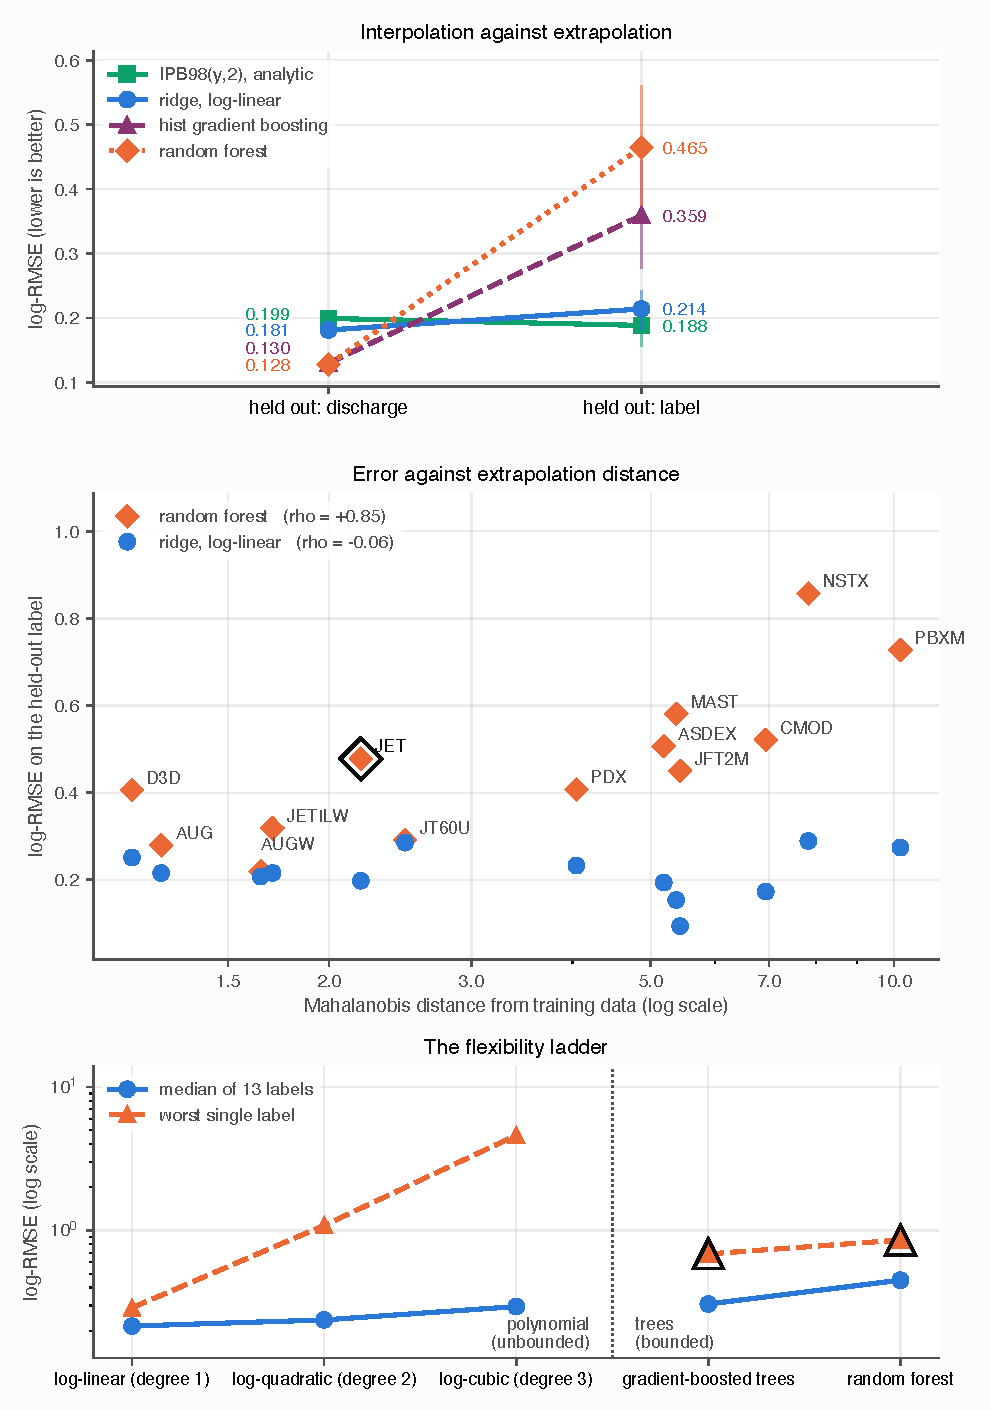
\includegraphics[width=\linewidth]{extrapolation}
\caption{\textbf{Interpolation against extrapolation.} Top: each model under
both splits, with bars giving the 95\% interval over the 13 held-out labels;
the lines crossing is the result. Middle: per-label error against Mahalanobis
distance from the training data, rising strongly for the random forest, more
weakly for the booster, and flat for the power law. The circled label is the second failure mode, where the true confinement
times run above anything the random forest can output. Bottom: the
flexibility ladder, where what grows with flexibility is the tail rather than
the centre; the circled points are the two tree ensembles, both observed here to
stay inside the training-target range, though only the random forest is provably
bounded to it.}
\label{fig:extrap}
\end{figure}

\subsection{Three diagnostics of the failure}
\label{sec:mechanisms}

\paragraph{Distance.} Ranking each model's per-label error against the
Mahalanobis distance of that label's mean log-feature vector from the
training mean gives $\rho=+0.85$ for the random forest and $+0.54$ for the
gradient booster, against $\rho=-0.06$ for the log-linear power law. The random
forest's error rises strongly with extrapolation distance and the gradient
booster's trends upward more weakly. The power law's does not: its error is
uncorrelated with how far the label sits from anything it saw.

Thirteen points is few enough that each of those numbers needs an uncertainty.
Permuting the distances 20000 times gives $p=0.0007$ for the forest, $p=0.060$
for the booster and $p=0.85$ for the power law. That permutation treats the 13
database labels as exchangeable, which they are not exactly: two physical
devices contribute two wall-era labels each, so these $p$-values are read as
Sec.~\ref{sec:data} says: summaries of how lopsided a count is. Recomputed over the 11 physical devices, which
removes the duplicated wall-era labels, the forest's correlation weakens slightly to
$+0.77$ ($p=0.005$) and the power law's is unchanged at $-0.06$ ($p=0.85$),
so the contrast the section rests on survives the collapse. That permutation
$p$-value is read the same way. The booster's falls
from $+0.54$ to $+0.38$ ($p=0.25$). Neither figure clears a conventional
threshold, and the booster's correlation is read throughout as suggestive rather
than established. Dropping each label in turn moves the forest's $\rho$ only
within $[+0.81,+0.88]$, so no single extreme device carries it. One control
changes how
the rest should be read: the \emph{mean baseline}, which fits nothing, also
correlates with distance, at $+0.56$. Distance predicts how hard a unit is in
general. What is unusual is not that the trees degrade with it but that the
power law does not.

\paragraph{The same distance in dimensionless coordinates.} Organising an
extrapolation audit by engineering variables invites one objection, and it is the
objection Hall \emph{et al.}~\cite{hall26} have raised in a conference
presentation: the weak size dependence in this database may come from a subset
localised in \emph{dimensionless} space rather than from size. Sec.~S12 of the
Supplementary Material repeats the distance construction above in
$(\rho^{*},\beta,\nu^{*})$, built from the same group definitions the
Connor--Taylor constraints of Sec.~\ref{sec:dimensional} are derived from and a
temperature recovered from the stored energy of Sec.~\ref{sec:robustness}. The
diagnosis translates: the two distance rankings agree at $\rho=+0.78$, and on
the rows a placement is possible for the forest's error tracks dimensionless
distance at $+0.77$ against $+0.79$ for engineering distance, with the power law
flat against both. The ITER-size-matched cut does not translate, and that half
goes to Hall: across it $\log\rho^{*}$ and $\log\nu^{*}$ separate as well as
size does, so that cut is a joint displacement in size, normalised gyroradius
and collisionality rather than a size boundary. Sec.~\ref{sec:size} says so, and
the leave-one-device-out comparison this paper rests on carries no such
confound.

Mahalanobis distance between mean log-feature vectors is one measure of how far
a unit sits from the training set, and it is the only one used here. It
compares first moments through a single pooled covariance, so it is insensitive
to differences in the shape or spread of a unit's operating envelope at a
fixed mean, and the covariance it uses is singular by Sec.~\ref{sec:rank} and so
is inverted through the pseudo-inverse. Every statement below about ``distance''
is a statement about that one diagnostic, not about distributional difference in
general.

The per-label scores behind that correlation are in Sec.~S8 of the
Supplementary Material.
On the five most distant labels (PBX-M, NSTX, C-Mod, JFT-2M and MAST, all
small, two of them spherical) the forest's error is $2.7$ to $4.8\times$ the
power law's; on the four nearest it is within $1.7\times$. JFT-2M and MAST sit
within 1\% of each other in distance, so the boundary is drawn to be
insensitive to that.

\paragraph{A hard bound, and the one fold it binds on.} A random forest predicts
by averaging leaf values, and every leaf value is itself a mean of training
targets, so every prediction it can make lies in
$[\min y_{\text{train}}, \max y_{\text{train}}]$ whatever the features say. With
JET held out, 48\% of its rows exceed the maximum confinement time anywhere in
the training fold, and its largest held-out target is $3.7\times$ above anything
any tree in the forest can output. More rows would close this only if they
carried larger targets: within the same target range no amount of additional
data, and no tuning, moves a ceiling that is a property of the functional form.

That is one fold of thirteen, and where the bound is active is reported here
rather than left to be found, because it decides which reading of
Sec.~\ref{sec:gp} this diagnostic supports. JET is the only held-out label whose
targets reach the ceiling at all. On the other twelve the largest held-out
target sits below it, by 1.31 in logs on JET-ILW and by 3.27, a factor of 26, on
MAST; \texttt{results/boundedness.json} carries the margin for every fold. The
size cut of Sec.~\ref{sec:size} is the second place it binds, and there
\textbf{34\%} of held-out rows lie above the ceiling.

Set against the per-label gaps, that pattern is evidence, and it points away
from the bound rather than toward it. The four labels the forest loses by the
widest margins are NSTX ($+0.568$), PBX-M ($+0.453$), MAST ($+0.427$) and
JFT-2M ($+0.357$), and on each of them its ceiling stands about three natural
logs above anything the held-out machine reaches. JET, the one fold where the
ceiling is in the way, is seventh of the thirteen by margin, at $+0.280$. The
forest therefore fails hardest where the bound is furthest from binding, and a
constraint that is not active cannot be what an error is made of. What is left
has to operate in the interior of the training range: predictions that stop
tracking the features once the input leaves the support the model was fitted on,
whether or not a ceiling is anywhere nearby. Section~\ref{sec:gp} builds the
model that separates the two readings and finds the second one, and this is the
first evidence in the paper that points there.

A gradient booster carries no such guarantee. It sums tree outputs onto an
initial estimate rather than averaging targets, and nothing in that
construction confines the sum to the training range, so the argument above does
not transfer to it. What can be reported is that it never uses the freedom: over
the 13 leave-one-out folds and the size cut of Sec.~\ref{sec:size}, its largest
prediction stays below $\max y_{\text{train}}$ on every one, coming closest with
JET held out at 0.066 in logs beneath the ceiling and sitting 0.567 beneath it
across the size cut. Its boundedness on these rows is measured rather than
guaranteed, and every claim below that needs the guarantee is made about the
forest.

\paragraph{Flexibility costs the tail, not the centre.} A polynomial ladder in
the log features (degrees 1--3) is flexible but still extrapolates. Degree 2 is
\emph{not} meaningfully worse than degree 1 on a typical label: median 0.238
against 0.216, better on 8 of 13, paired interval $[-0.013,+0.237]$ containing
zero. What flexibility costs is the tail. Degree 1's worst label is 0.289;
degree 2's is 1.083 and degree 3's is 4.601, both on C-Mod. A bounded range is
simultaneously why neither ensemble extrapolates and why neither blows up:
their worst cases, 0.686 and 0.857, sit far below degree 3's.

Read together, these three diagnostics invite a summary this paper does not
endorse. Every flexible model scored so far is also either bounded, like the two
ensembles, or divergent, like the cubic, so nothing above can tell apart
``flexible models fail out of distribution'' from ``models that stop trending
outside their data fail out of distribution''. The two make identical
predictions about everything in Table~\ref{tab:reversal}.
Section~\ref{sec:gp} builds the model that separates them and supports the
second interpretation, so the reader should carry the flexibility reading as
provisional from here rather than as the paper's conclusion.

\subsection{Sensitivity to population, aggregation, and device definition}
\label{sec:robustness}

Table~\ref{tab:reversal} attributes a difference to the split, so anything else
that differs between its two columns is a confound. Three things do. Grouped CV
scores all 6228 rows while leave-one-out scores only the 13 labels large
enough to hold out. Grouped CV pools out-of-fold predictions into one log-RMSE over
every row, where JET and AUG dominate, while leave-one-out averages per-label
scores, where every label counts once. And JET and JET-ILW are one physical
tokamak either side of a wall change, as are AUG and AUGW, so holding out
JET-ILW while training on JET does not hold out an unseen device.

\paragraph{The labels too small to score.} Five labels hold fewer than 30 rows
and none can carry a held-out score of its own, but all five stay in every
training fold, since the threshold governs scoring rather than training. They
are among the most unusual points in the feature space, so whether a flexible
model exploits them is a fair question; dropping them from training as well
leaves the ordering over the 13 held-out labels unchanged, and Sec.~S11 of the
Supplementary Material gives the arm.

\begin{table}[t]
\centering
\small
\caption{The random forest and the power law under both row populations, both aggregations,
and both definitions of a machine. The inversion is the pattern of the random
forest leading under cross-validation and trailing the power law under
leave-one-out; it holds in all eight combinations.}
\label{tab:robustness}
\begin{tabular}{lrrrr}
\toprule
& \multicolumn{2}{c}{pooled over rows} & \multicolumn{2}{c}{each unit equally} \\
\cmidrule(lr){2-3}\cmidrule(lr){4-5}
Split & forest & ridge & forest & ridge \\
\midrule
CV, all 18 labels          & 0.128 & 0.181 & 0.149 & 0.238 \\
CV, the 13 scored labels   & 0.123 & 0.177 & 0.124 & 0.187 \\
leave-one-label-out (13)   & 0.410 & 0.214 & 0.465 & 0.214 \\
leave-one-device-out (11)  & 0.551 & 0.200 & 0.527 & 0.211 \\
\bottomrule
\end{tabular}
\end{table}

Table~\ref{tab:robustness} varies all three. The forest leads the power law
under every cross-validation cell and trails it under every leave-one-out cell,
so the inversion is a property of the split rather than of the population or the
aggregation. Collapsing the variants makes the forest's failure worse rather
than better: over 11 physical devices its mean gap over the power law grows from
$+0.251$ to $+0.315$, with a paired 95\% interval of $[+0.221,+0.408]$ against
$[+0.157,+0.342]$ over the labels, and it loses on 11 of 11. The published law's score is
almost unmoved by any of it, 0.188 to 0.184 per unit.

\paragraph{A newer published law.} IPB98(y,2) is the ITER reference but not the
most recent scaling fitted to this database family. ITPA20 and
ITPA20-IL~\cite{hdb5} were derived from DB5.2.3 and weaken the size dependence
considerably. Each is specified on the separatrix elongation at the geometric
axis, $\kappa$, where the delivered file carries the areal elongation
$\kappa_a = S/(\pi a^2)$ that IPB98(y,2) was fitted to. That mismatch is
measured rather than modelled: the full DB5.2.3 revision this paper already pins
carries \texttt{KAPPA} on every analysed row, so each law is scored on the
elongation it was fitted to, which is what makes the three comparable.
Substituting the delivered column instead moves ITPA20 by up to 0.018 and
ITPA20-IL by up to 0.022, enough to reorder ITPA20 against IPB98(y,2) per label;
Sec.~S13 of the Supplementary Material measures that cost and says why a shape
model is the wrong way to find it.

Evaluated analytically on the rows analysed here, ITPA20 scores 0.188 over all
rows, 0.191 per label and \textbf{0.177} across the ITER-size-matched cut;
ITPA20-IL scores 0.237, 0.269 and \textbf{0.165}, against IPB98(y,2)'s 0.199,
0.188 and 0.194. Both are below the power law refitted inside these folds at
that cut, which scores 0.278, and against the random forest's 0.938 and the
gradient booster's 1.072 there ITPA20 is better by factors of 5.3 and 6.1. The
row is not blind and is not offered as one: both were fitted to selections out
of DB5.2.3, so at the size cut they had seen the large machines the fitted
models are being asked to reach. What it carries is that no published power law
in this family lands anywhere near where the tree ensembles land, and that the
two fitted to this revision are the two that beat a refit of the same functional
form on these rows.

\paragraph{Do the features name the machine?} One objection is more serious
than the four below it, because it explains everything in
Table~\ref{tab:reversal} without any appeal to long-range behaviour. Four of the
nine features barely move once a device is fixed. Major radius carries
\textbf{0.1\%} of its log variance within devices, minor radius 1.1\%, inverse
aspect ratio 4.9\% and elongation 6.1\%. A random forest classifier recovers the
device from the nine log features at \textbf{99.9\%} under the same
discharge-grouped split used throughout, against a 42.3\% majority baseline. The
feature vector is very nearly a device name. Under grouped cross-validation a
tree can therefore split on those coordinates and fit a per-device offset, which
is a lookup table: worth a great deal in sample, and worth nothing on a machine
that is not in it.

Deleting those features is the obvious control and it cannot settle the
question, which is worth showing rather than asserting. Refitting on the four
features that do move within a device, plasma current, toroidal field, density
and loss power, the reversal disappears: the forest's interpolation margin
\emph{grows} to 50.3\% and it is worse than the power law on 6 of 13 labels and
5 of 11 devices, at mean gaps of $-0.033$ and $-0.018$. That looks decisive and
is not, because the deleted columns carry the size dependence, and the size
dependence is the thing the power law extrapolates through. The control removes
the suspected leak and the physics under test together, and the power law's
held-out score more than doubles, from 0.214 to 0.477. It tells us that the
reversal needs features carrying size. It cannot tell us whether it needs them
because they carry size or because they name the machine.

The dimensionless coordinates separate exactly those two things. In
$(\rho^{*},\beta,\nu^{*},q,\epsilon,\kappa,M)$ the size, field and density
dependence is retained while no coordinate is a device label: $\rho^{*}$ moves
26.6\% within a device, $\beta$ 35.4\%, $\nu^{*}$ 66.6\% and $q$ 70.4\%, against
major radius's 0.1\%. Regressing $B\tau_{E}$ on those seven groups, with the
same models and the same splits, the reversal survives. The forest wins
cross-validation by \textbf{28.9\%}, against 28.7\% on the engineering features,
and loses on \textbf{11 of 13} labels and \textbf{9 of 11} devices, at mean gaps
of $+0.074$ and $+0.130$. The margins are smaller than the engineering-space
ones and the direction and the counts are the same.

So the reversal is not an artefact of the features naming the machine. It is
also not established at the strength the engineering-space numbers suggest: a
part of that $+0.315$ is device identity, and $+0.130$ is what survives in
coordinates where identity is unavailable. Both numbers are reported, and the
dimensionless one is the smaller. Three limits attach to it, and the third
decides how it should be read. The temperature it needs comes from the stored
energy of the control above, so it is scored on 6214 rows rather than 6228.
$\epsilon$ and $\kappa$ still move only 5\% and 6\% within a device, so the
coordinates are cleaner than the engineering ones rather than clean. And that
temperature is recovered as $T\sim W_{\mathrm{th}}/(nV)$ rather than measured,
while the control above puts $W_{\mathrm{th}}/(\tau_{\mathrm{th}}P)$ at a median
of unity on these rows, so the three groups are algebraic functions of the
target: substituting the definitions of Eq.~\eqref{eq:groups}, with
$V\sim Ra^{2}\kappa$, gives
$\log(B\tau_{E}) = \log\beta - \log P + \log V + 3\log B$ up to that ratio.
Two things follow. Neither model is blind in this arm in the way it is in the
engineering one, since each is handed a function of the held-out machine's own
confinement time. And these coordinates cannot be evaluated for a machine that
does not exist, because placing one needs the $\tau_{E}$ being predicted, which
is why the forecast of Sec.~\ref{sec:forecast} is stated in engineering
variables. This arm is a different experiment carrying a different confound
rather than a stricter version of the same one, and nothing below reads it as
the stricter one. The specification is in
\texttt{analysis\_dimensionless.py}.

\paragraph{Four choices that do not carry it.} Four more arms vary choices the
comparison had to make and that a reader could reasonably suspect of carrying
it. Sec.~S11 of the Supplementary Material gives each in full; the outcomes are
that none of them does. Sweeping the 30-row eligibility threshold over 10, 20,
30 and 50 rows changes only which labels are scored and never which are trained
on, and the power law wins every scored label at 20, 30 and 50 and 14 of 15 at
10. Repeating the cross-validation over ten shuffled fold assignments puts the
forest's interpolation margin between 27.0\% and 28.5\%, with the deterministic
partition's 29.5\% just above that range, so the margin it later gives up is not
a property of one partition. A nested hyperparameter search moves the forest's
settings in 13 of 19 folds and improves its held-out label score from 0.465 to
0.403, or 0.376 with the inner folds grouped by machine to match deployment,
against the power law's 0.214; at the size cut it makes the forest worse. And
dropping the spherical tokamaks, which IPB98(y,2)'s own selection excluded,
leaves the forest worse than the power law on all 11 remaining labels.

\paragraph{The loss power is the target's denominator.} The thermal confinement
time is the thermal stored energy over the thermal loss power, so
$\log\tau_{\mathrm{th}} = \log W_{\mathrm{th}} - \log P_{\mathrm{LTH}}$ up to
the deposit's $\mathrm{d}W/\mathrm{d}t$ and radiation conventions, and
$P_{\mathrm{LTH}}$ is one of the nine features every model sees. One predictor
is the denominator of the response. A log-linear model can carry the $-1$
coefficient on $\log P$ exactly, and carry it outside the training range of $P$
without error, because the relation is definitional rather than fitted; a tree
approximates it by axis-aligned splits and, by the bound of
Sec.~\ref{sec:mechanisms}, cannot extrapolate it at all. That admits a reading
in which the power law transfers because an identity is exactly log-linear
rather than because it has better long-range structure.

Refitting every model on the eight remaining engineering features tests it, and
the answer is a real qualification rather than a clean acquittal. The direction
survives and the strength does not. The forest still wins cross-validation, by a
wider margin than before, 0.198 against 0.316 where it was 0.128 against 0.181,
and it still loses under leave-one-label-out. But it loses on \textbf{10 of 13}
labels rather than 13, and \textbf{9 of 11} devices rather than 11, the exact
tests move to $p=0.092$ and $p=0.065$, from values that were small only under
the idealised null of Sec.~\ref{sec:data}, and the mean paired gap falls from
$+0.251$ to $+0.051$.
C-Mod, JT-60U and JET-ILW change hands, and the gradient booster's mean gap
turns negative, so with $P$ removed it beats the power law on average across
held-out labels. What survives is the direction: under both feature sets the
model that wins the interpolation comparison is the one that loses the
extrapolation comparison, which is the claim Sec.~\ref{sec:reversal} makes.

\paragraph{The same objection, answered the right way round.} Deleting $P$
answers more than the objection asks. $P$ is a real predictor of confinement as
well as the target's denominator, and deleting it removes both, which is most of
why the ablation above costs so much. The control the objection actually calls
for moves $W_{\mathrm{th}}$ to the left instead: regress $\log W_{\mathrm{th}}$
on the same nine features, so that $P$ stays among them as an ordinary predictor
and only the identity goes.

That control is available. STD5 carries no stored energy, but the full DB5.2.3
revision, already pinned by SHA-256 and analysed in
Sec.~\ref{sec:replication}, carries \texttt{WTH}, and joining it to STD5 on
machine, shot and time recovers one for \textbf{6214} of the 6228 analysed rows.
Two checks confirm the join: \texttt{KAPPAA} is delivered in both files and the
two copies agree to $5\times10^{-10}$, and on the joined rows
$W_{\mathrm{th}}/(\tau_{\mathrm{th}}P)$ has a median of 1.000000.

Retargeted, the direction and most of the magnitude survive; the unanimity does
not. The forest still wins cross-validation, 0.123 against the power law's
0.193. Under leave-one-label-out it loses on \textbf{9 of 13} labels at a mean
gap of $+0.220$, against 13 of 13 and $+0.251$ on $\tau_{\mathrm{th}}$; under
leave-one-device-out it loses on \textbf{9 of 11} at a mean gap of
\textbf{$+0.348$}, which is larger than the $+0.315$ the confinement time gives.
Across the ITER-size-matched cut it scores \textbf{1.081} against the power
law's 0.289, so the collapse the paper rests on is untouched. The exact tests
move to $p=0.267$ and $p=0.065$.

The two controls together separate what the identity carries from what it does
not. It carries the unanimity: under either control the count falls from
thirteen to nine or ten, and neither exact test then reaches $p=0.05$. It does
not carry the effect. Deleting $P$, which also deletes a genuine predictor,
leaves a mean gap of $+0.051$; deleting only the identity leaves $+0.220$ by
label and $+0.348$ by device and leaves the size cut where it was. A reading of
this paper as ``a log-linear model can represent $\tau = W/P$ exactly and a tree
cannot'' is therefore available, and this is the measurement that bounds what it
can carry.

This control is not what removing a term would do, which is why it is the
stronger one. Since $\log W_{\mathrm{th}} = \log\tau_{\mathrm{th}} +
\log P_{\mathrm{LTH}}$ and $\log P$ is a column of the design matrix, the matrix
is unchanged and one coefficient moves: the fitted exponent on $\log P$ goes
from -0.688 to $+0.308$, one unit, the identity carried on the other side
rather than taken away. The slope a tree has to reproduce in that direction more
than halves, so the control makes the tree's task easier, and the gap widens
anyway. The specification is in \texttt{analysis\_stored\_energy.py} and
\texttt{results/stored\_energy.json}.

Two results this paper leans on do not weaken. The interval collapse of
Sec.~\ref{sec:conformal} is unaffected in kind: on a held-out label at nominal
90\% the eight-feature intervals cover 42\% for the forest and 48\% for the
booster against 77\% for the power law, where the nine-feature figures are
35\%, 45\% and 83\%. Nothing about a conformal interval involves the target's
definition, and the measurement agrees. The kernel comparison of
Sec.~\ref{sec:gp} also holds: the bounded squared-exponential rung remains the
worst of the three processes, at 0.496 against 0.400 for the linear rung and
0.409 for their sum, where with $P$ it was 0.541 against 0.214 and 0.218. The
margin narrows and the ordering does not, and the linear-kernel process still
reproduces ridge to four decimals in both arms, which is the control that
licenses reading the rest.

The relation is not a defect in the feature set. It is physics, and it is the
physics Sec.~\ref{sec:dimensional} imposes deliberately: the Connor--Taylor
constraint on the exponent of $P$ is derived from $\tau_E = W/P$, and a
similarity transformation treating $P$ as an independent scale would produce a
constraint no published law satisfies. The constrained rungs therefore cannot be
scored under this ablation at all, since the constraint is defined over an
exponent vector that includes $P$.

\paragraph{The estimator this split design is usually paired with.} Every
comparison above sets a pooled global fit against ensembles, where the
clustered-validation literature cited here for the split design~\cite{roberts}
pairs it with a third kind of estimator: a mixed model carrying a random
intercept per device, from which a device never seen is predicted by the
population-level fixed effects alone. It is neither a power law nor a tree and
it is the fit matched to the deployment question, so Sec.~S10 of the
Supplementary Material fits and scores it rather than conceding it. It scores
\textbf{0.829} per device against the power law's 0.212, losing on 10 of the 11
devices, and sweeping its one variance component shows the best value that
component could take is the one at which the estimator \emph{is} the pooled
power law. What has been ruled out is narrower than the class: a single random
intercept, no random slopes, on eleven groups.

\section{A size-extrapolation stress test matched to ITER}
\label{sec:size}

Holding out JET still leaves the rest of the database spanning much of its range, so
leave-one-out extrapolates in identity while interpolating in size. ITER's major
radius is \SI{6.2}{\meter} against \SI{3.40}{\meter} for the largest row here, a
factor of 1.82. That factor is available inside the database: training on the 14
smallest database labels (up to DIII-D, \SI{1.865}{\meter}, 3498 rows) and predicting
the 4 largest labels (up to JT-60U, \SI{3.40}{\meter}, 2730 rows) demands a ratio of
1.823 against ITER's 1.824. The cut is selected by proximity to that ratio
rather than by eye, so it is a property of the data.

Two things bound what this cut can carry, and they are why it is a supporting
stress test here rather than the result the paper rests on. Its held-out side is
96\% JET: of 2730 rows, 1762 are JET and 866 JET-ILW, with JT-60U contributing
100 and TFTR 2. So it is close to a single-device holdout at a size ratio, not a
survey of large machines, and the per-label scores below matter more than the
pooled one because of it. And the boundary is drawn on major radius alone. Hall
\emph{et al.}~\cite{hall26} have argued, in a conference presentation, that the
weak size dependence in this database comes from a subset localised in
dimensionless space rather than from size as such, which is a different place to
cut. Sec.~\ref{sec:mechanisms} measures that
rather than conceding it, and the measurement goes their way: across this cut
$\log\rho^{*}$ and $\log\nu^{*}$ separate as well as size does. This section is
therefore transfer across a joint displacement in size, normalised gyroradius
and collisionality, not across size alone. The claim the paper rests on is the
leave-one-device-out result of Sec.~\ref{sec:reversal}, which does not depend on
where a size boundary is drawn.

\begin{table}[t]
\centering
\small
\caption{Three questions of increasing difficulty, scored in log-RMSE. The
\emph{size cut} column is the ITER-size-matched cut. Reading down it
rather than across the table is the point: the two models that win the first
column move far toward the constant baseline in the third, landing closer to it
than to the power law in absolute error.}
\label{tab:escalation}
\begin{tabular}{lrrr}
\toprule
Model & discharge CV & LOLO & size cut \\
\midrule
IPB98(y,2) & 0.199 & 0.188 & \textbf{0.194} \\
ridge, log-linear & 0.181 & 0.214 & \textbf{0.278} \\
random forest & 0.128 & 0.465 & \textbf{0.938} \\
hist grad.\ boosting & 0.130 & 0.359 & \textbf{1.072} \\
mean baseline & 0.869 & 0.994 & 1.459 \\
\bottomrule
\end{tabular}
\end{table}

Table~\ref{tab:escalation} places that cut beside the two easier splits. At
the cut the power law scores 0.278 against the analytic law's 0.194 and a
constant predictor's 1.459. The random forest scores 0.938 and the gradient
booster 1.072, so both sit nearer the constant than the power law in absolute
error. Asked the question a scaling law exists to answer, the two tree ensembles
that lead the conventional cross-validation comparison land closer to a constant
than to IPB98(y,2), the law they beat by 36\% under cross-validation and which
scores 0.194 here. The ordering is identical on all three
individually scored held-out labels, so the pooled number is not an artefact
of how JET is weighted within the pool.

That control is weaker than it looks, and the composition of the held-out side
should be read before the number is. The four labels above the cut are JET
(1762 rows), JET-ILW (866), JT-60U (100) and TFTR (2); TFTR falls far below the
30 rows required to report a label on its own and enters only the pooled number.
So 2628 of the 2730 held-out rows, \SI{96}{\percent} of them, come from a single
physical device, and the three individually scored labels are two physical
machines rather than three, since JET and JET-ILW are the same tokamak in two
wall eras. Seeing the same ordering twice on one machine is not two independent
confirmations of it. What this cut establishes is that the tree ensembles
collapse across an ITER-sized jump on the rows this database has above one, and
what would settle it is a second large device at comparable weight, which this
database does not contain. That is a limitation of the question as much as of
the split: large machines are few, and their scarcity is what makes the
extrapolation hard. This section rests on a large jump where
Sec.~\ref{sec:reversal} rests on many machines. Dropping the spherical tokamaks moves the
random forest from 0.938 to 0.936, so the effect is not driven by including the
spherical devices; other shape or regime covariates that track size are not
ruled out by this control.

\section{A power law with a bounded correction}
\label{sec:hybrid}

The diagnosis in Sec.~\ref{sec:mechanisms} suggests a repair that Sec.~S9 of the
Supplementary Material builds and scores: fit the power law, learn a correction
on its log residuals, and damp it, so that what the tree ensemble is bounded on
is a residual centred on zero rather than a target that grows with machine size.
Across the ITER-size-matched cut a bounded correction takes the power law from
0.278 to \textbf{0.206} while an unbounded polynomial correction takes it to
0.356, and the mechanism is measurable: the base law is biased on the held-out
machines and the correction points the right way and is largest where the bias
is largest.

Two limits keep this a supporting result rather than a recommendation, and both
are why it sits in the supplement. Cross-validation selects the most heavily
corrected rung in both families while the rung that transfers is the uncorrected
one, so a practitioner tuning on the split they would ordinarily use does not
arrive at it. And over the whole size sweep the bounded hybrid wins 5 of 8
well-powered cuts rather than all of them, with no rule separating the wins from
the losses. Anchoring a learned correction on a frozen power law is also the
design of concurrent work on this database~\cite{wang}, and nothing here is a
claim on that idea. The controlled version of the comparison, which holds the
nonlinear component fixed and varies only the long-range mean, is
Sec.~\ref{sec:meanfunction}.

\section{Calibrated intervals and their collapse}
\label{sec:conformal}

\begin{table}[t]
\centering
\small
\caption{Empirical coverage of nominal 90\% split-conformal intervals, and the
multiplicative half-width under leave-one-out.}
\label{tab:coverage}
\begin{tabular}{lrrrr}
\toprule
Model & CV & LOLO & ITER cut & width \\
\midrule
IPB98(y,2) & 90\% & 89\% & 88\% & 1.40$\times$ \\
ridge, log-linear & 90\% & 83\% & 70\% & 1.33$\times$ \\
bounded hybrid & 90\% & 64\% & 76\% & 1.26$\times$ \\
hist grad.\ boosting & 91\% & 45\% & \textbf{0\%} & 1.23$\times$ \\
random forest & 91\% & 35\% & \textbf{3\%} & 1.23$\times$ \\
\bottomrule
\end{tabular}
\end{table}

For a next-step device the point error is not the deliverable; the interval is.
Split-conformal intervals~\cite{conformal} are calibrated on log residuals,
holding back 25\% of \emph{discharges} to calibrate.

The construction is specified as follows, so that a reader can reproduce the
coverage numbers rather than infer the procedure from them. Within each training
fold, the distinct discharge identifiers are permuted with
\texttt{numpy.random.default\_rng} seeded at 20240811, and the first
$\mathrm{round}(0.25\,n_{\text{discharges}})$ of the permutation are the
calibration discharges; every row of a calibration discharge is a calibration
row, and the model is fitted on the remaining rows only. Arms with fewer than
100 calibration rows are not reported. The conformity score is the absolute log
residual $\lvert\log\hat\tau - \log\tau\rvert$. The half-width is the
$\lceil (n+1)(1-\alpha) \rceil$-th smallest score in ascending order, at
$\alpha=0.10$, which is the finite-sample conformal rank rather than the plain
empirical quantile; the $+1$ accounts for the test point itself being one of the
$n+1$ exchangeable scores, and where that rank exceeds $n$ the half-width is
reported as infinite rather than as a finite but invalid number. Ties need no
rule, since the quantile is a rank on a sorted array. The interval is
symmetric in $\log\tau$ and is a pointwise interval for a new observation, not
for a latent mean. Under grouped cross-validation the per-fold coverages are
pooled over rows; under leave-one-label-out each held-out label is
calibrated and scored on its own fold and the coverages are then averaged over
machines.

Holding out whole discharges keeps a calibration row and a test row from coming
out of the same shot, but the conformity unit is still the row, and rows arrive
in correlated clusters of quasi-stationary slices from one discharge. The
standard finite-sample guarantee assumes exchangeable conformity scores and
clustered rows do not supply that, so every coverage number below is empirical
row-level coverage rather than a guaranteed rate. A discharge-level conformity
score, or a cluster-aware conformal method of the jackknife+ and CV+
family~\cite{jackknife}, would be the way to recover a guarantee, and neither is
used here.

Interval estimation for a next-step device on this database family is not new:
Kardaun~\cite{kardaun} constructed confidence and prediction intervals for
ITER's confinement time from the predecessor database, by a parametric route
rather than a distribution-free one. What is asked here is narrower, and is
about a procedure rather than about ITER: whether an interval calibrated the
conventional way still covers once the held-out unit is a device.

That proviso is what the section measures. Empirical coverage is near nominal under grouped
CV, where every model lands within a point of 90\%, and that control is what
licenses reading the rest of Table~\ref{tab:coverage}. It is a useful
in-distribution control rather than a verified guarantee: clustered row-level
conformity scores do not satisfy the finite-sample exchangeability condition
either, so what the CV column shows is that the construction behaves as intended
when the test rows come from labels the model has seen. The exchangeability
assumption is no longer justified when the test rows come from a systematically
held-out label absent from the model's training and calibration distribution,
and what that costs empirically is measured below. That exchangeability is the
binding assumption, and that repairing it requires knowing the shift, is the
subject of the weighted-conformal literature~\cite{shiftcp}, and calibrated
uncertainty degrading under dataset shift is a general finding rather than a
fusion one~\cite{ovadia}. The random forest's 90\%
interval then covers 35\% of rows on an unseen label and 3\% across the
ITER-size-matched cut; the gradient booster covers \textbf{8} of the 2730 rows
there, which is 0.3\%.

A coverage that close to zero is worth checking against arithmetic before it is
read as a finding, because a calibration bug would produce the same number. The
booster's half-width across that cut is 0.221 in logs, calibrated on the rows
below it, and its per-label errors above it run from 0.66 to 1.13. A typical
residual is therefore three to five times the half-width, and an interval of
that size has no opportunity to contain the point. The coverage is not a
separate fact from the point errors of Table~\ref{tab:escalation} but the same
failure read on a different scale, and the two agree.

The widths barely move: no model's interval changes width by more than
1.5\% between the two arms. That is forced rather than found, and it is worth
being explicit about which part of it is a measurement. The half-width is the
$\lceil (n+1)(1-\alpha)\rceil$-th smallest calibration score, calibration rows
are drawn the same way in both arms, and a rank statistic of those scores has no
route by which the test distribution could reach it. So the width was never
going to move, and the residual 1.5\% is fold-to-fold noise in which rows land
in calibration. What is measured is the coverage, and what the fixed width
means for a reader is the point: the interval carries no signal that it has
stopped covering, so it cannot be inspected for the failure it is exhibiting. Figure~\ref{fig:conformal} shows
both halves of that: the coverage of every model under each split against the
nominal line, and the per-label coverage against extrapolation distance.

\begin{figure}[!htbp]
\centering
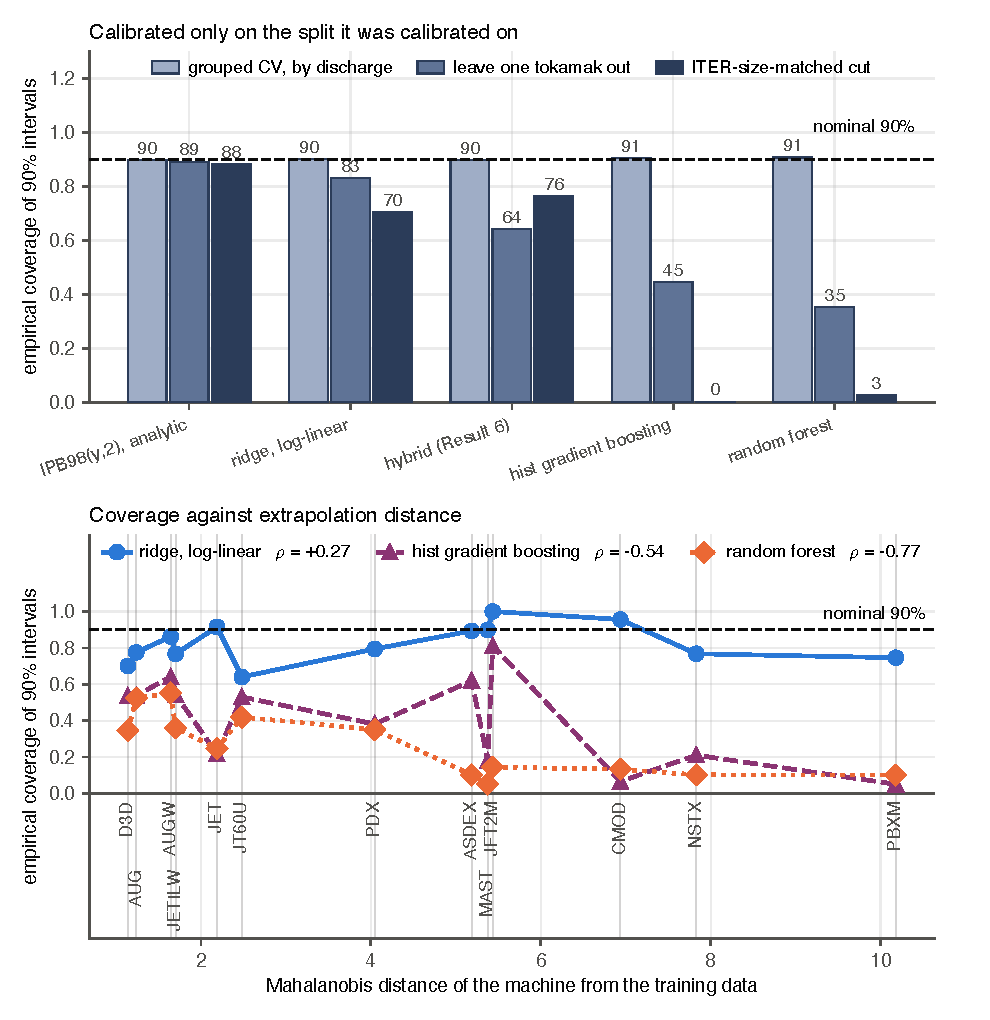
\includegraphics[width=\linewidth]{conformal}
\caption{\textbf{The interval collapse.} Top: empirical coverage of nominal
90\% split-conformal intervals for each model under the three splits, against
the nominal line. Every model is calibrated under grouped cross-validation, and
only the linear and constrained fits stay near it once the held-out unit becomes
a whole label and then a size range. Bottom: per-label coverage against the
Mahalanobis distance of the label from the training data. Under grouped
cross-validation coverage is flat on the nominal line at every distance; under
leave-one-label-out the tree ensembles fall away with distance and the power law
does not. Interval widths behind both panels move by under 1.5\% between the
splits, so what is drawn is intervals that keep their size and lose their
coverage.}
\label{fig:conformal}
\end{figure}

Coverage collapses along the same axis the errors grow, but only for the trees:
$\rho=-0.77$ for the random forest and $-0.54$ for the gradient booster against
$+0.27$ for the power law, mirroring the per-label error correlations of Sec.~\ref{sec:mechanisms}
with the sign flipped. The power law's intervals are somewhat too narrow
everywhere rather than catastrophically too narrow far away, and for a
next-step device that distinction is most of what matters, because distance is
the one thing known in advance. None of this is a defect in
conformal prediction. It is a measurement of an assumption being false.

\section{Dimensional constraints from Connor--Taylor similarity}
\label{sec:dimensional}

Every model to this point learns its functional form from the data. None is
told any physics. That is worth revisiting, because the field has known since
Connor and Taylor~\cite{connor} that a confinement scaling law is not free:
requiring it to be expressible in the dimensionless plasma variables imposes
\emph{linear equality constraints on the exponents}. The experimental programme
built on that identity is long-standing, and the constraints used here are the
same ones it works in: dimensionless-parameter scaling experiments hold the
dimensionless groups fixed and vary the remaining scale, which is the
transformation family derived below, run on a machine~\cite{petty,luce}. What is new here is not the constraint but where it
is imposed, as an equality on a fitted surface scored out of distribution. A physics assumption is
therefore a matrix $C$, and the fit becomes
\begin{equation}
\min_{b}\ \lVert Xb - y \rVert^{2} \quad \text{subject to} \quad Cb = d ,
\end{equation}
which the Karush--Kuhn--Tucker (KKT) system solves in closed form. Nothing new is needed to run the
experiment: the solver is the one written by hand for Sec.~\ref{sec:refit}.

The constraints are derived in code from the definitions of $\rho^{*}$, $\beta$
and $\nu^{*}$ rather than transcribing exponents from a paper, which makes the
derivation checkable against something external. Written as exponents on
(length, field, temperature, density),
\begin{equation}
\rho^{*} \sim T^{1/2} B^{-1} L^{-1}, \qquad
\beta \sim n\,T\,B^{-2}, \qquad
\nu^{*} \sim n\,L\,T^{-2},
\label{eq:groups}
\end{equation}
and a law expressible in whichever of these a model holds fixed must be
invariant under every scale transformation that leaves those groups unchanged.
Each such transformation contributes one linear equation in the exponents, so
the admissible set is a surface and the number of constraints is set by how many
groups are fixed, as Table~\ref{tab:hierarchy} sets out.

\begin{table}[!ht]
\centering
\small
\caption{The Connor--Taylor hierarchy. Each row fixes a set of dimensionless
groups and contributes one linear equation in the exponents per admissible
scale transformation, so fixing fewer groups imposes more constraints.}
\label{tab:hierarchy}
\begin{tabular}{lcc}
\toprule
constraint & groups held fixed & rows of $C$ \\
\midrule
Kadomtsev~\cite{kadomtsev} & $\rho^{*}$, $\beta$, $\nu^{*}$ & 1 \\
collisionless & $\rho^{*}$, $\beta$ & 2 \\
electrostatic & $\rho^{*}$ & 3 \\
\bottomrule
\end{tabular}
\end{table}

\noindent Fixing fewer groups admits more transformations and therefore imposes
more constraints, which is why the hierarchy runs the way it does. $C$ and $d$
are built by \texttt{dimensional.constraint\_matrix} from
Eq.~\eqref{eq:groups} alone, and their numerical rows are in
\texttt{results/dimensional.json}.

Constraining a confinement scaling this way is not new, and IPB98(y,2) is
itself an instance of it: the high-$\beta$ Kadomtsev constraint was enforced
when it was fitted, alongside a magnetic-field exponent fixed at
0.15~\cite{ipb98,hdb5}. Its exponents accordingly land on the Kadomtsev
surface~\cite{kadomtsev} derived here at a distance of 0.00096, and on the
collisionless surface at 0.0045. The first of those is expected rather than
surprising, and it is used only as a check that the surfaces derived in code
from Eq.~\eqref{eq:groups} agree with the constraint the published law was
fitted under. What is new here is not the idea of constraining the exponents
but the comparison: a hierarchy of such surfaces, fitted and scored under a
validation protocol matched to the deployment problem.

\paragraph{Where the newer published laws sit on these surfaces.} That check
invites a harder one, which the same machinery runs and which this section
should not decline to report about its own subject. The two laws of
Sec.~\ref{sec:robustness} that transfer best across the ITER-size-matched cut
are also the two furthest from every surface derived here. Their triangularity
term is dimensionless and contributes no column to $C$, so the eight exponents
the constraint is written over compare directly.

\begin{table}[!ht]
\centering
\small
\caption{Distance from each Connor--Taylor surface, as
$\lVert Cb-d\rVert$ over the eight exponents the constraint is written over,
beside the score each set of exponents gives across the ITER-size-matched cut.
The two published laws fitted to this database revision are the two furthest
from every surface and the two best across the cut. The numerical rows are in
\texttt{results/dimensional.json}.}
\label{tab:surfacedistance}
\begin{tabular}{lrrrr}
\toprule
exponents & Kadomtsev & collisionless & electrostatic & ITER cut \\
\midrule
IPB98(y,2), published      & \textbf{0.00096} & 0.0045 & 0.501 & 0.194 \\
free refit (this database) & 0.0031 & 0.064 & 0.817 & 0.279 \\
ITPA20, published          & \textbf{0.0147} & 0.089 & 0.745 & \textbf{0.177} \\
ITPA20-IL, published       & \textbf{0.0142} & 0.106 & 0.853 & \textbf{0.165} \\
\bottomrule
\end{tabular}
\end{table}

Proximity to a surface therefore does not order these four, and no claim here
rests on reading it that way. ITPA20 sits fifteen times further from the
Kadomtsev surface than IPB98(y,2) and scores 0.177 against 0.194 at the cut, and
the free refit sits closer to that surface than either ITPA20 law while scoring
0.279, the worst of the four. A small residual is not a predictor of transfer on
this evidence.

What the hierarchy measures is narrower than that, and it is measured the only
way a constraint can be: against a refit on these rows where the constraint is
the single difference, the same nine features, the same closed-form solver and
no hyperparameter separating 0.279 from 0.183. Table~\ref{tab:surfacedistance}
is about four different fitting populations and cannot weaken a comparison
internal to one.

It does point at what else a fitted law has available, and that is this paper's
own argument arriving from the fitting side rather than the scoring side.
ITPA20-IL is fitted to an ITER-like selection out of DB5.2.3 rather than to the
whole of it, which is what its name denotes. Sec.~\ref{sec:intro} asks that a
validation split match the deployment being claimed; restricting the fitting
population to the regime being extrapolated \emph{to} is the same principle
applied to the fit rather than to the score, and across this cut it is worth
more than any constraint tested here. The two are not competing repairs. A
constraint is what a fit can carry when the population cannot be restricted,
which is the situation of anyone refitting the published database as this paper
does; the ITER-like selection is a choice the ITPA authors could make and this
analysis could not, since the machines defining that regime are the ones held
out. Both supply structure that the rows alone do not, which is the section's
claim, and neither is evidence that the other is unnecessary.

The three rungs do not carry the same evidential status, and separating them
matters more than ranking them does. The Kadomtsev rung is
\emph{prospective}. It was specified by Kadomtsev in
1975~\cite{kadomtsev}, and enforced when IPB98(y,2) was fitted in
1998~\cite{hdb5}, both without reference to anything measured here; imposing it
is a prediction this analysis inherited rather than a surface it selected. The
collisionless rung is the best of the three at the size cut and was selected on
that basis; what the selection costs the claim is set out where the number is
reported. The prospective one comes first below.

\begin{table}[t]
\centering
\small
\caption{Fitting under the Connor--Taylor constraint hierarchy, ordered by
score at the ITER-size-matched cut. The only difference between the first and
last rows is the constraint: same features, same solver, no hyperparameter. The
Kadomtsev row is the prospective one, fixed by the literature before this
analysis; the collisionless row was selected on the scores in this table. LODO
is the same held-out score over the 11 physical devices rather than the 13
database labels, so it is the arm Sec.~\ref{sec:robustness} argues the paper
rests on, applied here to the models this paper recommends rather than only to
the ones it criticises. \emph{Worse on} counts the physical devices in that arm
on which a row scores above the unconstrained fit, and is the same per-unit
statistic this paper counts with wherever it criticises a model; the last row
calibrates it.}
\label{tab:dimensional}
\begin{tabular}{lrrrrcr}
\toprule
Model & in sample & CV & LOLO & LODO & worse on & ITER cut \\
\midrule
power law, collisionless & 0.1818 & 0.182 & 0.206 & 0.203 & 5/11 & \textbf{0.183} \\
IPB98(y,2), analytic$^{*}$ & n/a & 0.199 & 0.188 & 0.184 & 4/11 & 0.194 \\
bounded hybrid (Sec.~\ref{sec:hybrid}) & n/a & 0.151 & 0.246 & 0.246 & 5/11 & 0.206 \\
power law, electrostatic & 0.2245 & 0.225 & 0.241 & 0.226 & 8/11 & 0.237 \\
power law, Kadomtsev & 0.1808 & 0.181 & 0.210 & 0.211 & 7/11 & 0.254 \\
power law, unconstrained & 0.1808 & 0.181 & 0.214 & 0.212 & 8/11$^{\dagger}$ & 0.279 \\
\bottomrule
\end{tabular}
\\[2pt]
{\footnotesize $^{*}$historical reference, fitted to the DB2.8 predecessor of
this database~\cite{hdb5} and not refitted within these folds. The
unconstrained row is the closed-form least-squares fit this section's solver
produces, at 0.2790 across the size cut; the ridge spelling of the same power
law reported elsewhere gives 0.2778, and Sec.~\ref{sec:rank} shows the choice
between them carries nothing. $^{\dagger}$This row's count is that same pair
compared against each other, two solvers for one model, and is the calibration
for the column rather than a result.}
\end{table}

Take the prospective rung first. The Kadomtsev constraint is \emph{free}: at
0.1808 in sample it matches the unconstrained fit to four decimals, because the
data already satisfies it unaided. It nonetheless beats that unconstrained fit
at every one of the 15 cuts in the size sweep, including all 8 well-powered
ones, where a cut is called well-powered when it trains on at least 1000 rows.
Satisfying a constraint on average is not the same as being unable to violate
it, and what the constraint buys is a fit that cannot wander along that
direction when the training half is small or shifted. The underpowered rungs
show it directly: at six training machines the unconstrained fit scores 0.971
and the Kadomtsev fit 0.274. Nothing in that comparison was selected after the
fact, which is why it is the result in this section to weigh most heavily.

That rung owes a count as well as a score. This paper reports a per-unit win
count wherever it criticises a model, and the same statistic is available for
the models it recommends: over the 11 physical devices the Kadomtsev fit is
worse than the unconstrained one on \textbf{7} of them, at a mean paired
difference of 0.001 in its favour, and the collisionless fit is worse on
\textbf{5}, at 0.009 (\texttt{results/device\_arm.json}). Neither count is
evidence that a constraint hurts, and the last row of
Table~\ref{tab:dimensional} is the calibration that says why: the unconstrained
fit scored against the ridge spelling of the same power law, two solvers for one
model separated by 0.00008 per device, is worse on 8 of the 11. At the gaps
separating the rows of this table a per-device count is a coin toss, and none of
them carries what the 11 of 11 of Sec.~\ref{sec:reversal} carries. What survives
the observation is the size sweep, where the gaps are an order of magnitude
larger: the honest summary is that a constraint pays where the training half is
small or shifted, and sits inside the resolution of Sec.~\ref{sec:limitations}
where it is not.

The collisionless rung is the stronger assumption and the better score.
Something can still be said for it that does not depend on the score. It is a physics judgement about the machine being extrapolated
\emph{to} rather than a hyperparameter: one adopts it because one expects the
target plasma to be collisionless, and ITER is expected to sit at lower
normalised collisionality than the devices in this database rather than higher.
That points at this rung in advance, for a reason external to the data. The rung
also has no within-surface quantity to tune, so there is nothing for a
validation split to fit even in principle. Neither observation makes the result
prospective, and the disclosure stands as written.

At the ITER-size-matched cut the collisionless power law scores \textbf{0.183}, the
lowest held-out error of any model fitted here without using the held-out rows
(Table~\ref{tab:dimensional}). That qualifier excludes the published laws, and
two of them are lower: ITPA20-IL scores 0.165 there and ITPA20 0.177
(Sec.~\ref{sec:robustness}), both having been fitted to selections out of the
revision analysed here and so having seen the machines above the cut. Nothing
below is a claim to have beaten them. The fit is blind to the held-out rows; the
\emph{search} is not. No coefficient ever saw a held-out row, but the constraint
rung was chosen after seeing how each of the three scored at this cut, so the
cut took part in model selection even though it never entered a fit. This is
therefore the lowest error among the surfaces examined, not a prospective
demonstration that the collisionless surface is the right one. It beats the
bounded hybrid of Sec.~\ref{sec:hybrid}, which was built specifically for that
cut, and it beats the analytic law, which was fitted under a Kadomtsev
constraint of its own on a predecessor database. Figure~\ref{fig:dimensional} shows the trade between what each
constraint costs in sample and what it buys at the size cut.

The collisionless constraint costs 0.001 in sample against the unconstrained
fit and wins at 8 of 8 well-powered cuts, so it is not a single lucky cut, but
it is worse than Kadomtsev at every rung below the well-powered line: it is the
stronger assumption and it pays only where there is enough data for constraining
to be worth doing. Push one rung further to a
beta-independent law and it degrades sharply, to 0.237. There is an optimum in
the middle of the hierarchy, and nothing in this analysis predicted where it
would fall; as with the hybrid, cross-validation does not select it. Every
constrained fit scored slightly worse than the unconstrained one under the
cross-validation used here, so CV supplies no signal pointing at the constraint
that transfers best. That is an observation about these folds rather than a
theorem: a hard equality constraint can only match or worsen the \emph{training}
residual, and nothing forces it to worsen a held-out score.

It matters that this is a constraint and not a prior. Supplying the same physics
as a Gaussian prior instead, shrunk along the weak singular direction of
Sec.~\ref{sec:refit}, is worth much less. That comparison sweeps three
shrinkage geometries (isotropic, spectral and truncated) over the same nine
penalty strengths $10^{-3}, 10^{-2}, \dots, 10^{5}$, tabulated in full in
\texttt{results/dimensional\_prior\_sweep.csv}. Targeting the shrinkage beats
isotropic shrinkage at every one of those matched penalty strengths, which is a
real effect, but nothing in that family beats simply adopting IPB98's published
exponents outright. The hard
constraint used here restricts the fit to a surface the Connor--Taylor
similarity assumptions permit, where
the Gaussian prior tested here favours a location and a direction in parameter
space, and in this experiment the surface transfers better. That is a statement
about these two families rather than about priors in general: a prior can favour
a subspace, and approaches a hard constraint as its variance goes to zero.

\begin{figure}[!htbp]
\centering
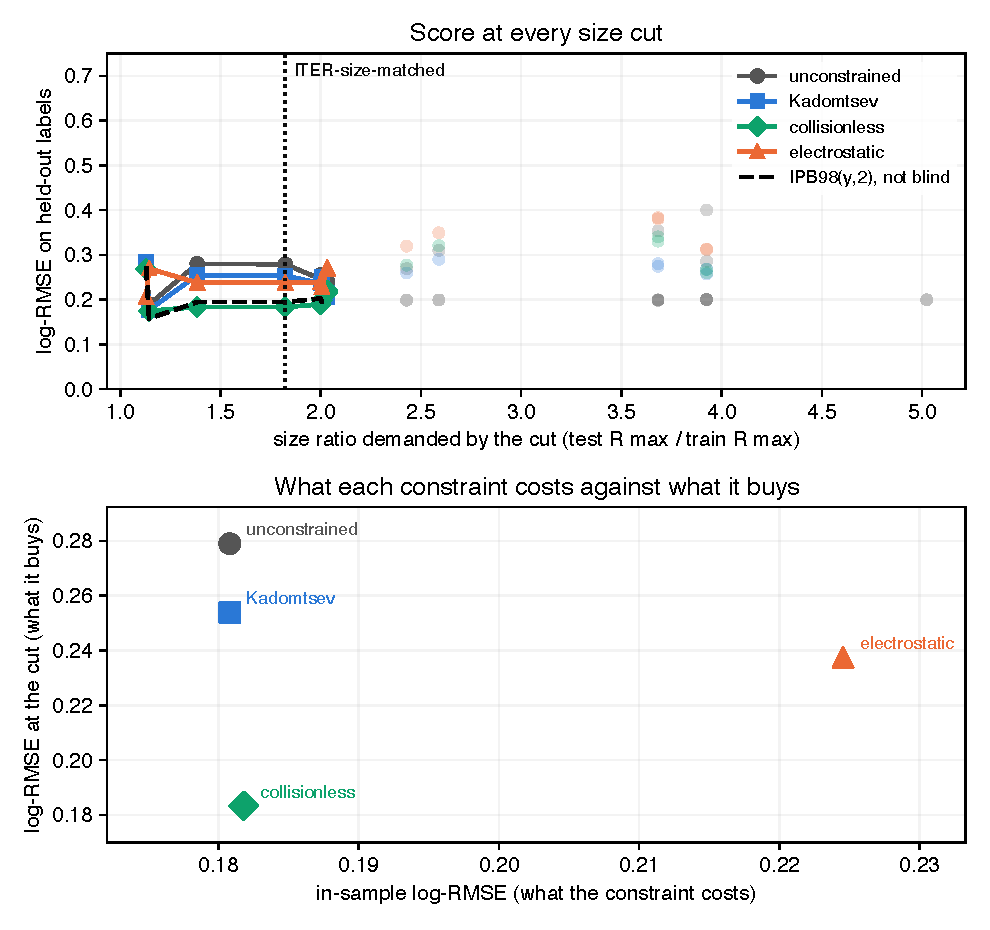
\includegraphics[width=\linewidth]{dimensional}
\caption{\textbf{Cost against benefit across the size sweep.} Top: the score at
every size cut for the constrained and unconstrained fits, with underpowered
cuts drawn faint and excluded from claims. Bottom: what each constraint costs in
sample against what it buys at the ITER-size-matched cut. The constraint costs almost
nothing where the data is plentiful and pays where it is not, and more physics
is not monotonically better: the hierarchy has an optimum in its middle, at the
collisionless rung, which was itself selected on these scores.}
\label{fig:dimensional}
\end{figure}

\section{Repairing the intervals, and the limit of the repair}
\label{sec:shift}

The diagnosis in Sec.~\ref{sec:conformal} makes a testable prediction. If the
collapse is about exchangeability rather than about the models, then calibrating
on held-out \emph{labels} instead of held-out discharges should repair it, and
should repair it only as far as that unit reaches. Both halves hold. On a
held-out label, empirical row-level coverage returns to within two points of
nominal for every model, the random forest going from 35\% to 88\%. Across the
ITER-size-matched cut none of the schemes tested restores it, because every
calibration unit is smaller than every test unit, and scaling the interval by
extrapolation distance recovers only part of the gap, 3\% to 40\% for the
forest.

Repeating the whole procedure over the 11 physical devices, which removes the
overlap that leaves JET in the calibration set when JET-ILW is the target, shows
the repair is less complete than the label-level numbers suggest: the booster
reaches 77\% by device against 90\% by label, and the trees buy their coverage
at 2.3 to 2.8$\times$ multiplicative half-width where the linear models stay
near 1.4$\times$. Among the models refitted within folds, the constrained power
law of Sec.~\ref{sec:dimensional} is the only one whose plain split-conformal
coverage stays near nominal at the size cut, at 91\%, and its intervals hold
there under every scheme.

Section~S1 of the Supplementary Material gives both calibration schemes in full,
the two coverage tables, and the reasons neither scheme is a
finite-sample-valid group-conformal procedure.

\section{Robustness on rows the standard analysis set excludes}
\label{sec:replication}

Everything above rests on one file, which is a central limitation of the
preceding analysis. The same OSF project publishes the full DB5.2.3 revision,
14153 rows against STD5's 6228, pinned by its own SHA-256. Matching on
(tokamak, shot, time) shows STD5 is an ELMy-H-mode quality selection out of it,
and leaves two populations this study had not analysed: 5358 H-mode rows STD5
does not contain, across 12 labels with zero row overlap, and 3860 ohmic and
L-mode rows in a different confinement regime, scored against
ITER89-P~\cite{iter89p} because an H-mode law is the wrong baseline for an
L-mode plasma.

The ranking inverts in both arms, and it survives dropping the 336 discharges
the disjoint H-mode arm shares with STD5 at different time slices. Counting
label--model pairs where a tree ensemble loses to the published law on an unseen
label gives 19 of 24 and 10 of 10. Counted instead against the power law
refitted inside each fold, which Sec.~\ref{sec:intro} calls the like-for-like
baseline and which the rest of this paper states the reversal against, it is
\textbf{16 of 24} and \textbf{9 of 10}; both counts are reported because the
second is the one this paper's own standard asks for. Section~S2 of the Supplementary Material
reports both arms in full, with the positive and negative checks on the row
matcher, whose silent failure would otherwise reproduce
Sec.~\ref{sec:reversal} by construction. This is emphatically \emph{not} an
independent database: both arms come from the same ITPA collection and the same
devices, and the five-machine arm is too small to carry a claim alone.

\section{A locked forecast, and a direction that is not size}
\label{sec:forecast}

Everything above is retrospective. To make the disagreement checkable rather
than merely described, what each model predicts for three real devices, SPARC,
JT-60SA and ITER, is recorded with intervals, a lock date of 31 August 2026 and
a content digest over the input rows, so that a later edit to them is visible.
The parameter sets are published design values, and none of the three has a
\emph{measured} H-mode thermal confinement time at the operating point
tabulated, which is what makes these predictions rather than retrodictions.
Section~S3 of the Supplementary Material gives the table, the interval
construction, the disclosures attaching to it and the falsification conditions;
the locked values are in \texttt{results/forecast.json}. It is a record rather
than a validation, and only JT-60SA is checkable in the near term. On JT-60SA,
which sits inside the database's size range and is already operating, all five
models agree to within 15\%. On ITER, $1.82\times$ beyond it, they disagree by a
factor of \textbf{8.3}, and for the random forest that gap cannot be closed by
tuning: its prediction cannot exceed the largest training target,
\SI{1.321}{\second}.

The disagreement among the models that \emph{can} reach ITER is the one a design
study would act on, and quoting it as a range hides it. The constrained power
law of Sec.~\ref{sec:dimensional} predicts \SI{2.837}{\second} at the $Q=10$
inductive point and the unconstrained refit \SI{2.858}{\second}, against
IPB98(y,2)'s \SI{3.591}{\second}: the two fits made here are \textbf{21\%} below
the reference law at the operating point it was used to size. That is the only
number in this paper a next-step design would consume, and four things bound
how much weight it can take. It is a point estimate from a fit selected on
transfer rather than on physics; the constrained rung it comes from was chosen
after the size-cut scores had been seen, so its standing is the one
Sec.~\ref{sec:dimensional} gives it; it points the same way as the newer
published laws, which weaken the size dependence relative to IPB98(y,2) and
which Sec.~\ref{sec:robustness} finds transferring better here than either fit;
and the operating point is the $Q=10$ inductive scenario of the 1999
basis~\cite{ipb98}, whose eight engineering values the 2007 revision carries
forward for the same scenario~\cite{doyle07}, since when ITER has been
rebaselined on a schedule this paper does not attempt to
summarise~\cite{loarte}, so the row is conditional on the operating point
tabulated in Sec.~S3 rather than on ITER's current plan of record.

One feature of the exercise was not anticipated by anything above. SPARC sits
\emph{further} from the training data than ITER does, at a Mahalanobis distance
of 6.9 against 4.7, despite being the smaller machine: its \SI{12.2}{\tesla}
field is 2.1 times the largest toroidal field anywhere in the cleaned STD5 rows,
\SI{5.82}{\tesla} on Alcator C-Mod, and every other label tops out at or below
\SI{4.80}{\tesla}. Size is not the only direction in which a next-step device
leaves the data behind, and an extrapolation audit organised around size alone
would have missed it.

\section{Flexibility, or long-range saturation?}
\label{sec:gp}

Section~\ref{sec:mechanisms} left two readings open, and every model scored to
this point confounds them. Flexibility is how much structure a model can learn
beyond a power law; \emph{saturation} is whether its predictions stop tracking
the features once the input leaves the training support, either because they
cannot leave a fixed range or because they revert to a fixed value. The forest
is the strict case, provably confined to
$[\min y_{\text{train}}, \max y_{\text{train}}]$; the booster never left that
range on any split scored here; a squared-exponential Gaussian process reverts
to its prior mean. What the three share is the absence of a trend that continues
outside the data. The ensembles are flexible and saturating, ridge is neither,
and the degree-3 polynomial is flexible and non-saturating but divergent, which
is why its worst label is 4.601. Nothing scored so far is flexible,
non-saturating and well behaved at long range at once.

A Gaussian process (GP)~\cite{gpml} supplies one, and the property is a choice
of kernel rather than a tuning parameter. The tool is not new to this field:
Chilenski \emph{et al.}~\cite{chilenski} fit plasma profiles and impurity
transport coefficients this way for the uncertainty a parametrised fit does not
honestly give, which is a different use from the one here, where what the kernel
is chosen for is its behaviour far outside the data rather than its error bars
inside it. Section~S6 of the Supplementary
Material fits three
over the same log features, with the same optimiser on the same rows, differing
in whether the kernel admits a trend that continues at long range, and the
ordering is the one saturation predicts. The squared-exponential rung alone
scores 1.948 at the ITER-size-matched cut, worse than a constant predictor, its
error tracking distance at $\rho=+0.65$. Adding a dot-product term gives the
best cross-validated score in this work, 0.112 against the forest's 0.128,
together with 0.191 at that cut and an error flat against distance at
$\rho=-0.01$. Its intervals behave differently from the calibrated ones as well,
which is taken up below.

That ladder suggests the mechanism without isolating it, because a dot-product
term enlarges the function class as well as changing the asymptote. The rest of
this section removes that objection.

\subsection{The same experiment with the nonlinear component specified identically}
\label{sec:meanfunction}

Write the model as a mean function plus a residual process,
\begin{equation}
\log\tau = m(x) + g_{\text{RBF}}(x),
\label{eq:meanfunction}
\end{equation}
and specify $g$ identically in every arm: same RBF covariance family, same
tuning subsample, same seed, same optimiser. Only $m$ changes. The fitted
processes are not the same function, because each is conditioned on its own
mean's residuals and each re-optimises its hyperparameters on those. What is
held fixed is the nonlinear capacity available to the model and the procedure
that fits it, so no part of the difference below can come from one arm having
more of either.

Two arms would not be enough. An RBF residual decays to zero over a finite
length scale, so far outside the training support the prediction \emph{is} the
mean function and its score \emph{is} the mean function's score; comparing a
constant mean against a fitted power law therefore cannot separate ``saturation
is the mechanism'' from ``whatever mean you supply is what you get out here'',
and only the second would be demonstrated. The third arm separates them. Its
mean also keeps trending, and its slope is IPB98(y,2)'s, fixed in 1998 and
fitted to nothing here, so two of the three arms have a trend and differ only in
which trend it is.

\begin{table}[t]
\centering
\small
\caption{One RBF covariance family and fitting procedure, three mean functions.
The constant-mean row reproduces the squared-exponential rung of Sec.~S6 of the
Supplementary Material to six decimals, which is the control: the decomposition
is the same model rewritten. Only the first row saturates. The other two both
keep trending, and they do not agree, which is what makes this an ablation
rather than an identity. The LODO column repeats the held-out score over the 11
physical devices, where the three separate more widely than they do over the 13
labels.}
\begin{tabular}{lrrrr}
\toprule
$m(x)$ in Eq.~\eqref{eq:meanfunction} & CV & held-out & LODO & ITER cut \\
\midrule
constant & 0.142 & 0.541 & 0.693 & 1.948 \\
fitted power law & 0.115 & 0.212 & 0.212 & 0.278 \\
IPB98(y,2), unfitted & \textbf{0.112} & \textbf{0.189} & \textbf{0.186} & \textbf{0.186} \\
\bottomrule
\end{tabular}
\label{tab:meanfunction}
\end{table}

Table~\ref{tab:meanfunction} reports the three arms. Take the control first:
with a constant mean, Eq.~\eqref{eq:meanfunction}
returns 0.141533, 0.540967 and 1.947535, which is the RBF row of
that rung to every digit computed. Nothing has changed except how the
model is written. Giving the
same process a power-law mean then moves the ITER-size-matched cut from 1.948 to
0.278, a factor of 7.0, and improves the cross-validated score as well, 0.115
against 0.142. Because the residual GP has the same covariance family, the same
capacity and the same fitting procedure in both rows, the difference cannot be
attributed to adding nonlinear model capacity.

The second row's cut score is worth reading closely: 0.277823 is plain ridge's
score at that cut, to six decimals. Far outside the data the RBF residual has
reverted to its training mean, which for a ridge mean is zero, and the model
falls back to its mean function. A saturating model reverts to something; the
failure of the squared-exponential rung is that a constant mean makes that
something a constant, and the repair is not to make the model less flexible but
to give it something worth reverting to.

The third row is what stops that being a tautology. If the only content of this
section were that the model returns its mean function far from the data, then
any trending mean would do equally well and the two trending rows would land
together. They do not. Swapping the fitted power law for IPB98(y,2)'s published
exponents, with nothing else changed, moves the cut from 0.278 to
\textbf{0.186}, improves the held-out label score from 0.212 to 0.189 and the
cross-validated score from 0.115 to 0.112. Having a trend is necessary and it is
not sufficient: which trend decides the answer, and out here the answer is the
trend and nothing else. That the best of the three is a law fitted in 1998 to a
predecessor database, on exponents this study did not choose, is the same
observation Sec.~\ref{sec:robustness} makes about the published laws, arriving
from a different direction.

Three numbers in this paper answer to the description ``a linear trend with a
bounded correction'', and they differ, so it is worth saying how. The two
trending rows above fix the trend first, by penalised least squares in one case
and by adopting published exponents in the other, and give the residual process
no say in it; they score 0.278 and 0.186 at the cut. The linear-plus-RBF kernel
of Sec.~\ref{sec:gp} instead fits both components jointly by maximising the
marginal likelihood, and scores 0.191. None of the three is a disagreement about
the mechanism, which all of them exhibit. What separates them is where the trend
comes from, and on this database the trend that transfers best came from outside
the fit entirely. The kernel is marginally the best cross-validated model here,
at 0.11179 against the IPB98-mean arm's 0.11196, which is a tie at any precision
worth quoting; out of distribution the two part company, 0.218 against 0.189 on
a held-out label. None of the three beats the constrained fit of
Sec.~\ref{sec:dimensional} at 0.183, and the two that come near it, at 0.186 and
0.191, sit inside the 0.01 resolution Sec.~\ref{sec:limitations} states, so they
are tied with it rather than behind it. Sec.~\ref{sec:robustness} reports two
published laws below all of them.

Across the model families tested here, this resolves the choice
Sec.~\ref{sec:mechanisms} left open: extrapolation failure tracks long-range
saturation rather than flexibility alone. The set of models in
Sec.~\ref{sec:reversal} is measured correctly, and every flexible member of it
was either bounded or divergent, so nothing in it could have separated the two
properties; that is why the reading there was flagged as provisional rather than
asserted. ``Do not use a flexible model out of distribution'' is the wrong
lesson. ``Do not use a model whose predictions stop tracking the features once
the input leaves the training data'' is the right one, and the random forest's
training-target ceiling is its strictest case. This does not displace the
constrained power law, which ties it across the ITER-size-matched cut, 0.183
against 0.191, a difference inside the resolution of
Sec.~\ref{sec:limitations}, and which carries no within-surface hyperparameter
to tune; and the process does not beat the
power law on a held-out label (0.218 against 0.214). Held out one physical
device at a time, which is the arm Sec.~\ref{sec:robustness} argues for, it
scores 0.219 against the power law's 0.211 and is worse on 5 of the 11. So the
process ties the power law under the stricter split as it does under the looser
one, and the statement that it does not reverse is made on the split this paper
says the claim belongs to rather than only on the finer partition.

A Gaussian process also supplies an interval by construction rather than by
calibration, so Sec.~\ref{sec:conformal}'s question
can be put to a model that was never calibrated. At the ITER-size-matched cut, at
nominal 90\%, the flexible unbounded rung covers 92.5\%, where split-conformal
intervals give the random forest 3\% and the gradient booster none. It is the
only flexible model tested whose \emph{native} posterior intervals reach nominal
coverage out of distribution without conformal recalibration. That is a
statement about where the interval comes from rather than about coverage alone:
the constrained power law of Sec.~\ref{sec:dimensional} also holds near nominal
at this cut (91\%, Sec.~\ref{sec:shift}), but through an externally calibrated
split-conformal interval rather than one the model supplies itself. The bounded rung is the instructive failure: it is the
one model that does become vague out of distribution, with a half-width four
times any other, and it still covers 16.7\%, having reverted to a prior mean
nowhere near the answer. Width was never the problem.

\section{Discussion}
\label{sec:discussion}

The practical consequence of Table~\ref{tab:reversal} is narrow and specific.
It is not that machine learning has nothing to offer confinement scaling, and
not that the models scored here are badly built. It is that conventional
within-database evaluations do not measure the quantity the law is used for.
Cross-validation grouped by discharge, or by shot, or by time slice, holds out
rows from machines that remain in the training set. It measures interpolation within known devices.
A scaling law is used to size a device that does not exist, which is
extrapolation to an unknown one, and on this database the two comparisons do not
merely differ in magnitude: they order the candidate models in opposite
directions. A gain reported under the first is not evidence about the second.

This is the selection argument of Sec.~\ref{sec:intro}, now measured, and it
has to be stated at the width the evidence carries. Over the three primary models
scored here, all of which saturate, the convention does not merely fail to
inform about extrapolation: it picks the worst of the three extrapolators on
offer, and the more carefully it is followed the more confidently it does so.
How far that generalises depends on how much of the literature on this database
also fits saturating models, and this paper does not measure that. Tree
ensembles are fitted to it~\cite{xiong}; whether a variational or
sampling-based Bayesian neural network~\cite{gao}, or a deep ensemble under
feature alignment~\cite{namseo}, saturates is a question about those
architectures that only scoring them under this split would settle, and a
network with a linear output layer would not. None of the four is scored here
and no claim is made about any of them. It is not a
property of cross-validation as such, and this paper holds its own
counterexample. Enlarge the candidate set with a model whose predictions keep
trending and the selection rule repairs itself. The linear-plus-RBF Gaussian
process of Sec.~\ref{sec:gp} is the best cross-validated model in this work, at
0.112 against the random forest's 0.128, and it is the flexible model that does
not collapse: 0.218 on a held-out label, which ties the power law's 0.214 rather
than beating it, and 0.191 across the ITER-size-matched cut against 0.278, with
a per-label error flat against distance ($\rho=-0.01$). A practitioner who put that model in the
comparison would be selected onto it. What fails is therefore not the score but
the set of models the score is applied to, and the property separating the
survivors from the casualties is long-range saturation, which
Sec.~\ref{sec:meanfunction} isolates and which can be read off an estimator
before any device is held out.

\subsection{What this changes in practice}

The consequence is primarily a reporting convention rather than a modelling one, and it is
short enough to state as a checklist. For any confinement model offered as an
alternative to a power law on this database:

\begin{enumerate}\setlength{\itemsep}{3pt}
\item Report leave-one-device-out beside cross-validation. It costs one refit
per device, on the same rows and the same features, and the two numbers print
together. Where they agree the interpolation number is informative. Where they
disagree, as here by a factor of 3.6, the disagreement is the result, and the
interpolation number should not be quoted on its own.
\item Report how far the target operating point sits from the training
distribution. The distance itself needs no held-out device and is the one
quantity known in advance for a machine that does not exist. Its
\emph{correlation} with error is not free in the same way: it is measured over
held-out units, so it arrives with item 1, and distance alone predicts how hard
a unit is rather than which model will fail on it, since the mean baseline of
Sec.~\ref{sec:mechanisms} correlates with it at $+0.56$ while fitting nothing.
What separates the models here is the contrast, $\rho=+0.85$ for the random
forest against $\rho=-0.06$ for the power law.
\item Say whether the model's predictions stop tracking the features outside the
training support, and separately whether they can leave the range of the
training targets at all. Both are properties of the estimator, checkable before
anything is fitted. The second is sharper and narrower: a random forest provably
cannot leave that range, since every prediction is an average of training
targets. On this database that bound is active on one held-out label of the
thirteen and across the size cut, and the forest loses worst on labels where it
is nowhere near binding, so it is the first of the two properties that carries
the failure here.
\item Do not carry a calibrated interval across a device boundary without saying
so, and do not read its width as evidence about that. Split conformal assumes
exchangeable conformity scores, and across a held-out device the assumption is
false. What it costs is not a wider interval but the same interval with the
coverage removed: 90\% nominal delivering 35\% on an unseen label and 3\% across
the size cut, at a width that moves by under 1.5\% because a half-width fixed by
the calibration rank cannot move. The interval is therefore the wrong place to
look for the warning, and the distance of item 2 is the right one.
\end{enumerate}

\noindent Only the first needs a refit, and item 2's correlation is measured on
what that refit produces. Items 3 and 4, and the distance in item 2, cost
nothing and are computable from the fitted model and the intended operating
point alone.

The positive findings point the same way, and both are about the far field
rather than about capacity. Constraining the exponents to a Connor--Taylor
surface and adding a linear component to a Gaussian process kernel are unrelated
operations, and both supply long-range structure. They are not equivalent in
what else they change: the constraint removes freedom from the fit, while the
linear kernel also enlarges the GP's function class, so that rung on its own
cannot separate the asymptote from the capacity. The mean-function ablation of
Sec.~\ref{sec:meanfunction} is the cleaner test, since there the nonlinear
covariance family and the procedure fitting it are held fixed and only the
long-range mean changes. It should still be read as a statement about the families
tested, not about flexible models in general.

For practice, the cheaper option was also the stronger one out of distribution. A
power law refitted on the same rows is a stronger baseline out of distribution
than any tree ensemble scored here, and it costs a single least-squares solve;
the estimator hardly matters, since ordinary least squares on the independent
columns reproduces the reported ridge to within 0.0012 on every split. Where a flexible model
is wanted, the evidence here favours one that keeps trending, and the
linear-plus-RBF Gaussian process was both the best cross-validated model in this
study, at 0.112, and the only flexible model whose native posterior intervals
reached nominal coverage out of distribution without conformal recalibration.
That coverage is measured across the ITER-size-matched cut, so it is
one-machine evidence in the sense Sec.~\ref{sec:limitations} gives; the constrained
power law reaches comparable coverage there through split conformal instead. Where a physics constraint is available, imposing it is close to free and helps
out of distribution. The rung the literature fixed in advance costs nothing in
sample and beats the unconstrained fit at all 15 cuts of the size sweep; the
other costs 0.001 and was the best-scoring blind fit at the size cut, having
been selected on it.

None of this is settled by one database, and every fusion result above rests on
one ITPA file. Two replications outside fusion are reported in Secs.~S4 and~S5
of the Supplementary Material, and the second of them establishes something
these rows structurally cannot. Its nested predictor ladder varies how many
predictors the models see while holding the rows, the splits and the model
specifications fixed, and finds the extrapolation failure at every rung,
including the rungs where the flexible model has no interpolation advantage to
lose. That is the harder case, and the one with no warning sign at all: a
practitioner running the conventional comparison there sees nothing wrong and
still cannot extrapolate. HDB5 cannot show it, because on these nine features
the flexible model always wins the interpolation split. Running the same audit on the published laws of those two
fields, Kleiber's exponent~\cite{kleiber} and the allometry of the BAAD
compilation~\cite{baad}, reproduces the extrapolation failure in both, while the
ranking inversion appears only where the flexible model first wins the
interpolation split. Secs.~S4 and~S5 carry the construction and the caveats.

\section{Limitations}
\label{sec:limitations}

What this database can resolve is worth stating once, because several
comparisons above are close. Two models whose per-label scores differ by less
than about 0.01 in log-RMSE should be read as tied here, which is roughly the
spread the bootstrap puts on a single label's score and roughly what a fold
assignment moves the cross-validated margin by. On that reading the Gaussian
process at 0.218 and the power law at 0.214 are tied, as the text says; ITPA20's
0.191 and IPB98(y,2)'s 0.188 are tied; and the orderings the paper does claim,
the forest's 0.465 against 0.214 and the size cut's 0.938 against 0.278, are an
order of magnitude clear of it. No ordering finer than 0.01 is asserted
anywhere, and none should be read into a table.

The refit population is not IPB98's, and the refit exponents should not be read
as a correction to it. Two machines (JET and ASDEX Upgrade with their variants)
supply 77\% of rows. Only 13 of the 18 database labels are scored under
leave-one-label-out; the
five excluded are the smallest and most unlike the rest, so the reported gap is
if anything optimistic. Thirteen labels is a small bootstrap and the paired
differences are the more reliable statistic.

The training-target bound of
Sec.~\ref{sec:mechanisms} is a theorem for the random forest and an observation
for the gradient booster: boosting sums tree outputs rather than averaging
targets, so nothing confines it to the training range, and what is reported
here is only that it stayed inside that range on all 14 splits scored. The ITER-size-matched cut reproduces
ITER's size ratio and nothing else: ITER is a burning plasma dominated by alpha
self-heating at a gain no row here approaches, so clearing this bar is necessary
and not sufficient. Its composition is the sharper limit and is restated here
because several results rest on it. Of the 2730 held-out rows, 2628 are one
physical device, and the three individually scored labels are two machines
rather than three. The conformal collapse of Sec.~\ref{sec:conformal}, the
bounded correction of Sec.~\ref{sec:hybrid}, the constrained fit's 0.183, the
Gaussian process's 0.191 and the mean-function ablation of
Sec.~\ref{sec:meanfunction} are all scored across it, so all five are one-machine
evidence about a large jump, and the claim that rests on many machines is the
leave-one-device-out result of Sec.~\ref{sec:reversal} instead. Nothing in this
database fixes that: a second large device at comparable weight is what the
comparison needs and what does not exist.

The per-label coverages in Sec.~\ref{sec:conformal} are proportions over as
few as 39 rows and carry binomial uncertainty of ten points or more; the pooled
contrasts are far larger than that noise, the within-column ordering is not. The
constraint hierarchy of Sec.~\ref{sec:dimensional} has an optimum in its middle that nothing here
predicted and that cross-validation cannot select, so the result is that a
constraint helps rather than that this constraint is the right one.

The
robustness arms of Sec.~\ref{sec:replication} are disjoint in rows but not
independent in provenance: both come from the same ITPA collection and the same
devices, and the five-machine arm is too small to carry a claim alone. The
H-mode arm is disjoint in rows and not, as first constructed, in discharges;
Sec.~\ref{sec:replication} reports the rerun with all 336 shared discharges
removed, which the reversal survives. The locked forecast of
Sec.~\ref{sec:forecast} is a record, not a validation; only JT-60SA can be checked against
measurement in the near term, that check requires an H-mode campaign rather than
the completed L-mode one and no date is put on when that arrives, and it is the one device of
the three that sits inside the database's size range.

The two biological replications carry their own limitations, stated in full in
Secs.~S4 and~S5 of the Supplementary Material: the metabolic-rate arm has one
predictor and eleven
groups that are phylogenetically related rather than independent, which the
comparative-biology literature handles with phylogenetically controlled
regression~\cite{felsenstein} and this paper does not, and the plant ladder is one
ordering of one selectively intersected set of predictors, so it establishes
that a crossing exists and that the inversion tracks it, not that three is a
threshold. Neither establishes a rate for anything.

Every power-law fit here treats the engineering parameters as measured without
error, which the confinement-scaling literature has objected to for as long as
these fits have been published, because the predictors carry real measurement
uncertainty. Kardaun~\cite{kardaun} treats the problem directly,
Cordey~\emph{et al.}~\cite{cordey} refit the database under it, and
Verdoolaege~\emph{et al.}~\cite{gls} give a geodesic least-squares regression
built to be robust to exactly the noise an ordinary least-squares fit assumes
away. None of the three is attempted here. Refitting Eq.~\eqref{eq:powerlaw} by
orthogonal distance regression, which spreads the error across the predictors
instead, moves the exponents enormously: up to 5.6 on the inverse aspect ratio,
with the major radius going from 1.58 to 5.40, and it more than doubles the
in-sample error, 0.454 against 0.181. Both are symptoms of one thing rather than
a better fit. With no per-variable measurement uncertainties published for this
database, an errors-in-variables estimator has nothing pinning it down along the
weak singular direction of Sec.~\ref{sec:refit}, which carries 0.3\% of the
design's variance, and it runs away along exactly that direction. So these are
least-squares exponents, an errors-in-variables fit would differ, and what is
reported here is a fact about the naive estimator rather than an answer to what
a credible measurement-error fit would give.

How many comparisons this paper makes is worth stating in one place, because
each is disclosed where it appears and none is added up. Across two split
families, three published laws, six fitted models, three constraint rungs, three
kernels, three mean functions, nine damping settings, fifteen size cuts, four
eligibility thresholds, ten shuffled partitions, two feature sets and two
targets, the number of out-of-distribution comparisons reported here is of order
forty, and every $p$-value among them is an exact sign test over at most
thirteen units under a null Sec.~\ref{sec:data} calls an idealisation. No
correction for multiplicity is applied and none would mean much on units this
dependent. The consequence is not that the descriptive results need one: the
gaps that carry this paper are an order of magnitude clear of its stated
resolution, and win counts of 13 of 13 and 11 of 11 are not marginal findings.
It is that the constructive results were selected from a large search, and
exactly one of them is prospective. The Kadomtsev rung was fixed by the
literature in 1975 and enforced when IPB98(y,2) was fitted; the collisionless
rung, the damping factor and the forecast's interval scheme were each chosen
after seeing a held-out score, and are labelled as such where they appear rather
than only here.

The mixed model of Sec.~\ref{sec:robustness} is scored on eleven devices, which
is few enough that its one variance component is poorly determined: REML places
$\lambda$ anywhere between 2.0 and 143 depending on which device is held out.
The sweep is reported for that reason and is what the conclusion rests on, since
it does not depend on the optimiser. It also carries a single random intercept
and no random slopes, so what has been ruled out is that a device-level
\emph{level} shift is the missing structure. Sec.~S10 of the Supplementary
Material takes the next specification as far as this database allows: a random
slope on the features carrying the size dependence is not identifiable, since
those features barely vary within a device, and on the four that do vary an
unseen machine is still predicted from the population-level slope. More broadly, what the results above
establish is that the ordering of these models reverses and that nothing scored
here displaces the pooled power law on an unseen device, which is not the same
as its being the best available predictor of one.

Every fit also weights
rows equally, so JET and ASDEX Upgrade set most of what each model learns even
though the target is transfer to a device neither resembles. Refitting every
model with each label weighted equally, reported in Sec.~\ref{sec:robustness},
costs the power law more than the forest and takes the win count to 12 of 13.
The row imbalance is therefore not the source of the power law's advantage, but
it is not irrelevant to its size either, and one weighting is not a
characterisation of how the result behaves under reweighting in general.

The Gaussian-process intervals of Sec.~\ref{sec:gp} are
equal-tailed posterior intervals on $\log\tau$ that include the fitted
observation-noise term and are exponentiated to $\tau$; that is the closest
available analogue of a conformal interval, which is also a statement about a
new observation rather than a latent mean, but the two are not the same
construction and the comparison should be read as such. Those kernels are tuned
by marginal likelihood on a seeded subsample of each training fold, with only
the hyperparameters coming from the subsample and the posterior then conditioned
on the whole fold,
which is stable across the range that was affordable (under 4\% in every
hyperparameter between 750 and 1500 rows) but is not a proof that the full-data
optimum agrees; and ``linear plus RBF'' is one reading of ``a power law with a
bounded correction'' among several, with an anisotropic kernel, a Matern kernel
and a linear part constrained as in Sec.~\ref{sec:dimensional} all untested. The
last of these is the obvious next experiment, since the constraint and the
kernel are the two things that work here and nothing has tried them together.

\section{Conclusion}

On real confinement data, the model that wins cross-validation by 29\% over a
log-linear power law refitted inside the same folds loses to that same power law
on all 13 held-out database labels and on all 11 physical devices once the JET
and ASDEX Upgrade variants are collapsed, and to the published IPB98(y,2) law as
well, which is the historical reference of Sec.~\ref{sec:intro} rather than a
fold-fitted competitor.

Those counts are unanimous because the loss power is among the nine features
and is also the target's denominator, which a log-linear model represents
exactly and a tree cannot. The two controls of Sec.~\ref{sec:robustness}
separate what that identity carries from what it does not: it carries the
unanimity and the exact tests, which fall below significance under either
control, and it does not carry the effect. The mean-function ablation of
Sec.~\ref{sec:meanfunction} then identifies the mechanism as long-range
saturation, which the three diagnostics on their own cannot separate from
flexibility. That ablation runs in the engineering coordinates, where several
features are close to device labels, so it establishes the mechanism in the
coordinates the literature fits in rather than in general; the reversal itself
survives the change to dimensionless coordinates, at a reduced margin. At the
size extrapolation that separates this database from ITER, the two tree
ensembles that lead the conventional comparison land closer to a constant
predictor than to the power law, and their nominal 90\% intervals cover 3\% and
0\% of the held-out rows at unchanged width. The inversion survives every
robustness arm of Sec.~\ref{sec:robustness}, so it is not an artefact of a
single bookkeeping choice. What the models disagree about is recorded rather
than argued: on a machine inside the database's size range they agree to within
15\%, and on ITER they differ by a factor of 8.3.

The repair that scored best is not additional model flexibility at all: it is a
dimensional constraint on the existing power law, and the two rungs tested carry
different weight. The Kadomtsev rung was fixed by the literature in 1975 and
enforced when IPB98(y,2) was itself fitted, so imposing it here selected
nothing, and it costs nothing in sample. Where it does not show is the
leave-one-out arms, on which it gains 0.004 by label and 0.001 by device against
that same fit, inside the resolution Sec.~\ref{sec:limitations} states; its
measurable benefit is confined to the size sweep, which
Sec.~\ref{sec:limitations} also notes is one machine above the matched cut. The collisionless rung gave the lowest error of any model fitted
here without using the held-out rows at the ITER-size-matched cut, but was
selected after those scores had been seen, so it is the lowest error among the
surfaces examined rather than a prediction that this surface is the right one.
Two published laws fitted to this database revision score lower there still
(Sec.~\ref{sec:robustness}), and they had seen the machines above the cut.

Two results temper the diagnosis and neither weakens the practical advice. In
the nested predictor ladder of Sec.~S5 the extrapolation failure persists at
every predictor count tested while the ranking inversion does not, because the
inversion needs the flexible model to win the interpolation split first: a field
whose scaling law has one predictor faces the same danger with no warning at
all. And separating flexibility from long-range saturation shows the failure
belongs to the second: holding the nonlinear component's specification fixed and
varying only the mean function moves the ITER-size-matched cut sharply
(Sec.~\ref{sec:meanfunction}), and the better arm lands on the power law's score
there, because far from the data its correction has reverted to zero and left
the trend behind.

The lesson is not that flexible models cannot be trusted beyond their data. It
is that a model whose predictions stop tracking the features once the input
leaves the training data is structurally unsuited to a problem where the target
itself has to leave that range. The two are easy to confuse because the flexible
models that win the conventional interpolation comparison here are the
saturating ones, while the non-saturating polynomial control becomes unstable in
extrapolation instead.

\section*{Acknowledgments}

This work uses the ITPA Global H-mode Confinement Database, assembled and
maintained by the ITPA Confinement Database and Modelling Topical Group and by
the teams operating the contributing tokamaks. The author thanks them, and the
authors of Ref.~\cite{hdb5}, for releasing the standard analysis set publicly:
an independent recomputation of this kind is possible only because they did.
The replications outside fusion use the BAAD compilation~\cite{baad}, released
under CC0, and the metabolic-rate compilation deposited on Figshare that the
Supplementary Material describes. Neither the ITPA group nor any contributing
team has reviewed or endorsed this analysis, and its conclusions are the
author's alone.

% IOP puts the generative-AI disclosure, the funding statement, the competing
% interests and the contributions inside Acknowledgements, and its policy names
% that section explicitly. They are therefore run-in paragraphs of the section
% above rather than sections of their own. Anonymisation cannot simply drop the
% whole section any more: tools/make_submission.py removes the credit prose and
% the contributions paragraph by name and keeps the three required declarations,
% and it still fails loudly if the generative-AI paragraph goes missing.
\paragraph*{Use of generative AI.}
Two generative AI systems were used in
preparing this work, and each is named with its version and its role.

Anthropic Claude Opus 5 (model \texttt{claude-opus-5}) assisted with developing,
debugging and executing author-specified analysis code in the accompanying
repository, and with drafting and editing passages of this manuscript.

OpenAI GPT-5.6 Sol was used to critique complete drafts against journal policy
and for scientific and historical accuracy, to support the literature review,
and to identify methodological issues and propose robustness checks. Several of
its suggestions were adopted after the author judged them worth pursuing. They
include the corrected account of how IPB98(y,2) was fitted, in
Sec.~\ref{sec:reversal} and Sec.~\ref{sec:dimensional}; the recomputation of the
distance correlation over the 11 physical devices in
Sec.~\ref{sec:mechanisms}; the device-level calibration of
Sec.~\ref{sec:shift}; and several of the references in Sec.~\ref{sec:refit} and
Sec.~\ref{sec:forecast}, which the author then located and checked against their
published records.

Neither system is an author. The author designed the study, decided which
suggestions to pursue, specified and implemented every analysis reported here,
verified every reported number against the generated artefacts, checked every
reference against its published record, and takes full responsibility for the
content, the conclusions and any error in them. No text was incorporated
without the author reading and verifying it.

\paragraph*{Funding.}
This research received no specific grant from any funding agency in the public,
commercial or not-for-profit sectors.

\paragraph*{Competing interests.}
The author declares no competing interests.

\paragraph*{Author contributions.}
Sole author, in CRediT terms. L. Salcedo: conceptualization, methodology,
software, validation, formal analysis, investigation, data curation, writing
(original draft), writing (review and editing), visualization, project
administration.

\section*{Data availability}

Four third-party datasets underlie this work. None is redistributed here; each
is fetched from its public source by a script in the repository and verified
against a pinned SHA-256 on load, so every number above refers to one specific
set of bytes rather than to whatever a host currently serves.

\begin{itemize}\setlength{\itemsep}{2pt}
\item \textbf{ITPA Global H-mode Confinement Database, standard analysis set
STD5 (DB5.2.3).} The basis of every fusion result. Openly available from the
OSF deposit \emph{International Global H-Mode Confinement Database}~\cite{osfdb},
described in Ref.~\cite{hdb5}. File \texttt{hdb5\_std5.csv}.
\item \textbf{The full DB5.2.3 revision.} Used only for the replication of
Sec.~\ref{sec:replication}, which scores rows STD5 excludes. It is a separate
download from the same OSF project (\url{https://osf.io/download/zhwa3/}) and is
not a superset this paper generated. File \texttt{hdb5\_db523.csv}.
\item \textbf{Mammalian basal metabolic rate.} The Figshare deposit of
Capellini, Venditti and Barton~\cite{capellini}. Used in the Supplementary
Material. File \texttt{allometry\_bmr.txt}.
\item \textbf{Biomass And Allometry Database (BAAD) v1.0.1.} Released CC0; the
data paper is Ref.~\cite{baad} and the archive analysed here is release
v1.0.1~\cite{baadrelease}. Used in the Supplementary Material. File
\texttt{baad\_data.zip}.
\end{itemize}

\noindent The pinned fingerprints are those of Table~\ref{tab:fingerprints}.

\begin{table}[!ht]
\centering
\scriptsize
\caption{SHA-256 of each third-party input, verified on load. A file whose bytes
differ from these is refused rather than analysed, so every number in this paper
refers to one specific set of bytes.}
\label{tab:fingerprints}
\begin{tabular}{ll}
\toprule
file & SHA-256 \\
\midrule
\texttt{hdb5\_std5.csv} & \texttt{67601c2da5c51f90cf6298ff499cccc7} \\
 & \texttt{4d09ac80c2b98c7dde0d8db3ebb9ac5b} \\[2pt]
\texttt{hdb5\_db523.csv} & \texttt{7a48e34379663e3e298924990f05cd8f} \\
 & \texttt{16b8581516bcfa7bb8f438f83ae80ab6} \\[2pt]
\texttt{allometry\_bmr.txt} & \texttt{ab22d9ae8f35e96d7fbf5d8e53053d64} \\
 & \texttt{7f0594d74f8917888169993ce668571e} \\[2pt]
\texttt{baad\_data.zip} & \texttt{0375f012475658c039e3dcef398951e8} \\
 & \texttt{f68cdeb5430eec8cd65548965496cfe2} \\[2pt]
\bottomrule
\end{tabular}
\end{table}

\noindent The locked forecast of Sec.~\ref{sec:forecast} also carries a
content digest over its input rows, so that a later edit to the operating
points is visible:
\begin{center}\scriptsize
\texttt{960d537ee3df8780afd2054e51d01a268} \\
\texttt{f8803aca64a830dba37fd1ff5319192}
\end{center}
\noindent All code, the full writeup with every table and limitation, and the
scripts that regenerate every number and figure in this paper and its
Supplementary Material are openly available under the MIT licence at
\url{https://github.com/lsalcedo100/FusionFlux}, and the exact version used for
this paper is archived with a persistent identifier~\cite{zenodo}. The analysis
code is pinned as firmly as its inputs: every number and figure above was
produced at commit
\begin{center}\scriptsize
\texttt{0e81f8d5c517f263db3d406ae1f0abc6a59753bc}
\end{center}
\noindent Every script verifies that fingerprint against the pin as it loads
the data and refuses to run when the two disagree, so no number above can have
been computed from a different revision of the database. Several of the JSON
outputs under \texttt{results/} also record the digest they verified, which
carries that provenance into the artefact itself.

The prose is bound to those artefacts in the same way.
\textbf{One hundred and twenty-five} of the numbers printed above, and \textbf{one
hundred and sixty-two} across this paper and its Supplementary Material, are tied by test
to the field of the generated file they came from, in both directions: if an analysis is rerun and its output moves, the
rendered value stops matching the printed one and the suite fails; if a number
in the text is edited, it stops matching the artefact. A figure that disagrees
with the file behind it therefore cannot survive a test run, which is the check
a reader would otherwise have to perform by hand.

\begin{thebibliography}{99}
\small\setlength{\itemsep}{0pt}\setlength{\parskip}{0pt}
% DOIs are single unbreakable words, so justifying around one leaves a line
% stretched past what TeX will accept quietly. Reference lists are set ragged
% right for exactly this reason.
\raggedright
\bibitem{ipb98} ITER Physics Expert Group on Confinement and Transport, ITER
Physics Expert Group on Confinement Modelling and Database and ITER Physics
Basis Editors, ``Chapter 2: Plasma confinement and transport,'' \emph{Nucl.\
Fusion} \textbf{39}, 2175 (1999).
\href{https://doi.org/10.1088/0029-5515/39/12/302}{doi:10.1088/0029-5515/39/12/302}
\bibitem{hdb5} G. Verdoolaege \emph{et al.}, ``The updated ITPA global H-mode
confinement database: description and analysis,'' \emph{Nucl.\ Fusion}
\textbf{61}, 076006 (2021).
\href{https://doi.org/10.1088/1741-4326/abdb91}{doi:10.1088/1741-4326/abdb91}
\bibitem{doyle07} E. J. Doyle \emph{et al.}, ``Chapter 2: Plasma confinement
and transport,'' \emph{Progress in the ITER Physics Basis}, \emph{Nucl.\
Fusion} \textbf{47}, S18 (2007).
\href{https://doi.org/10.1088/0029-5515/47/6/S02}{doi:10.1088/0029-5515/47/6/S02}
\bibitem{creely} A.J. Creely \emph{et al.}, ``Overview of the SPARC tokamak,''
\emph{J.\ Plasma Phys.} \textbf{86}, 865860502 (2020).
\href{https://doi.org/10.1017/S0022377820001257}{doi:10.1017/S0022377820001257}
\bibitem{citrin} J. Citrin \emph{et al.}, ``Real-time capable first principle
based modelling of tokamak turbulent transport,'' \emph{Nucl.\ Fusion}
\textbf{55}, 092001 (2015).
\href{https://doi.org/10.1088/0029-5515/55/9/092001}{doi:10.1088/0029-5515/55/9/092001}
\bibitem{meneghini} O. Meneghini \emph{et al.}, ``Self-consistent core-pedestal
transport simulations with neural network accelerated models,'' \emph{Nucl.\
Fusion} \textbf{57}, 086034 (2017).
\href{https://doi.org/10.1088/1741-4326/aa7776}{doi:10.1088/1741-4326/aa7776}
\bibitem{sparccore} P. Rodriguez-Fernandez \emph{et al.}, ``Predictions of core
plasma performance for the SPARC tokamak,'' \emph{J.\ Plasma Phys.}
\textbf{86}, 865860503 (2020).
\href{https://doi.org/10.1017/S0022377820001075}{doi:10.1017/S0022377820001075}
\bibitem{allen} L. Allen and C. M. Bishop, ``Neural network approach to energy
confinement scaling in tokamaks,'' \emph{Plasma Phys.\ Control.\ Fusion}
\textbf{34}, 1291 (1992).
\href{https://doi.org/10.1088/0741-3335/34/7/008}{doi:10.1088/0741-3335/34/7/008}
\bibitem{katesharbeck} J. Kates-Harbeck, A. Svyatkovskiy and W. Tang,
``Predicting disruptive instabilities in controlled fusion plasmas through deep
learning,'' \emph{Nature} \textbf{568}, 526 (2019).
\href{https://doi.org/10.1038/s41586-019-1116-4}{doi:10.1038/s41586-019-1116-4}
\bibitem{rea} C. Rea, R.S. Granetz, K. Montes, R.A. Tinguely, N. Eidietis,
J.M. Hanson and B. Sammuli, ``Disruption prediction investigations using machine
learning tools on DIII-D and Alcator C-Mod,'' \emph{Plasma Phys.\ Control.\
Fusion} \textbf{60}, 084004 (2018).
\href{https://doi.org/10.1088/1361-6587/aac7fe}{doi:10.1088/1361-6587/aac7fe}
\bibitem{zhu} J.X. Zhu \emph{et al.}, ``Hybrid deep-learning architecture for
general disruption prediction across multiple tokamaks,'' \emph{Nucl.\ Fusion}
\textbf{61}, 026007 (2021).
\href{https://doi.org/10.1088/1741-4326/abc664}{doi:10.1088/1741-4326/abc664}
\bibitem{degrave} J. Degrave \emph{et al.}, ``Magnetic control of tokamak
plasmas through deep reinforcement learning,'' \emph{Nature} \textbf{602}, 414
(2022).
\href{https://doi.org/10.1038/s41586-021-04301-9}{doi:10.1038/s41586-021-04301-9}
\bibitem{murari} A. Murari, M. Peluso, M. Gelfusa and I. Lupelli, ``Symbolic
regression via genetic programming for data driven derivation of confinement
scaling laws without any assumption on their mathematical form,''
\emph{Plasma Phys.\ Control.\ Fusion} \textbf{57}, 014008 (2015).
\href{https://doi.org/10.1088/0741-3335/57/1/014008}{doi:10.1088/0741-3335/57/1/014008}
\bibitem{wang} Z. Wang \emph{et al.}, ``Power-law-anchored residual learning
for H-mode energy confinement time in tokamaks: interpolation and
parameter-defined extrapolation,'' arXiv:2608.20684 (2026).
\href{https://doi.org/10.48550/arXiv.2608.20684}{doi:10.48550/arXiv.2608.20684}
\bibitem{butt} J. Butt, G. Verdoolaege, S. M. Kaye and E. Kolemen,
``Revisiting confinement scalings and fusion performance with a perspective
optimized for extrapolation,'' arXiv:2604.22728 (2026).
\href{https://doi.org/10.48550/arXiv.2604.22728}{doi:10.48550/arXiv.2604.22728}
\bibitem{namseo} H. Nam and J. Seo, ``Machine learning based energy confinement
time extrapolation via multi-tokamak database,'' \emph{Fusion Eng.\ Des.}
\textbf{221}, 115369 (2025).
\href{https://doi.org/10.1016/j.fusengdes.2025.115369}{doi:10.1016/j.fusengdes.2025.115369}
\bibitem{gao} E. Gao \emph{et al.}, ``Bayesian neural networks for predicting
tokamak energy confinement time with uncertainty quantification,''
\emph{Nucl.\ Fusion} \textbf{65}, 084001 (2025).
\href{https://doi.org/10.1088/1741-4326/ade8fd}{doi:10.1088/1741-4326/ade8fd}
\bibitem{xiong} X. Xiong, K. Zhang, Y. Gao, L. Zhang, X. Chen and S. Liu,
``Bayesian optimization based machine learning for predicting tokamak energy
confinement time with quantification of feature importance,'' \emph{Fusion
Eng.\ Des.} \textbf{227}, 115740 (2026).
\href{https://doi.org/10.1016/j.fusengdes.2026.115740}{doi:10.1016/j.fusengdes.2026.115740}
\bibitem{roberts} D.R. Roberts \emph{et al.}, ``Cross-validation strategies for
data with temporal, spatial, hierarchical, or phylogenetic structure,''
\emph{Ecography} \textbf{40}, 913 (2017).
\href{https://doi.org/10.1111/ecog.02881}{doi:10.1111/ecog.02881}
\bibitem{abbate} J. Abbate \emph{et al.}, ``Large-database cross-verification
and validation of tokamak transport models using baselines for comparison,''
\emph{Phys.\ Plasmas} \textbf{31}, 042506 (2024).
\href{https://doi.org/10.1063/5.0190908}{doi:10.1063/5.0190908}
\bibitem{meredig} B. Meredig \emph{et al.}, ``Can machine learning identify the
next high-temperature superconductor? Examining extrapolation performance for
materials discovery,'' \emph{Mol.\ Syst.\ Des.\ Eng.} \textbf{3}, 819 (2018).
\href{https://doi.org/10.1039/C8ME00012C}{doi:10.1039/C8ME00012C}
\bibitem{sutton} C. Sutton \emph{et al.}, ``Identifying domains of applicability
of machine learning models for materials science,'' \emph{Nat.\ Commun.}
\textbf{11}, 4428 (2020).
\href{https://doi.org/10.1038/s41467-020-17112-9}{doi:10.1038/s41467-020-17112-9}
\bibitem{breiman} L. Breiman, ``Random forests,'' \emph{Machine Learning}
\textbf{45}, 5 (2001).
\href{https://doi.org/10.1023/A:1010933404324}{doi:10.1023/A:1010933404324}
\bibitem{leyland} M.J. Leyland \emph{et al.}, ``The H-mode pedestal structure
and its role on confinement in JET with a carbon and metal wall,''
\emph{Nucl.\ Fusion} \textbf{55}, 013019 (2015).
\href{https://doi.org/10.1088/0029-5515/55/1/013019}{doi:10.1088/0029-5515/55/1/013019}
\bibitem{hall} J. Hall, P. Zhang and G. Verdoolaege, ``Confinement scaling with
machine size in the updated ITPA global H-mode energy confinement database,'' in
\emph{Proc.\ 49th EPS Conf.\ on Plasma Physics}, Bordeaux, Europhys.\ Conf.\
Abstr.\ \textbf{47A}, P1.024 (2023).
\bibitem{hall26} J. Hall, P. Zhang, Y. Zhang, C. Angioni and G. Verdoolaege,
``Confinement scaling with machine size in the updated ITPA global H-mode
energy confinement database,'' poster P2.1097, \emph{52nd EPS Conf.\ on Plasma
Physics}, Edinburgh (2026). Conference presentation; not published in refereed
form at the time of writing.
\bibitem{conformal} V. Vovk, A. Gammerman and G. Shafer,
\emph{Algorithmic Learning in a Random World}, Springer (2005).
\href{https://doi.org/10.1007/b106715}{doi:10.1007/b106715}
\bibitem{jackknife} R. Foygel Barber, E. J. Cand\`{e}s, A. Ramdas and R. J.
Tibshirani, ``Predictive inference with the jackknife+,'' \emph{Ann.\ Statist.}
\textbf{49}(1) (2021).
\href{https://doi.org/10.1214/20-AOS1965}{doi:10.1214/20-AOS1965}
\bibitem{kardaun} O. J. W. F. Kardaun, ``Interval estimation of global H-mode
energy confinement in ITER,'' \emph{Plasma Phys.\ Control.\ Fusion} \textbf{41},
429 (1999).
\href{https://doi.org/10.1088/0741-3335/41/4/001}{doi:10.1088/0741-3335/41/4/001}
\bibitem{shiftcp} R.J. Tibshirani, R. Foygel Barber, E.J. Cand\`es and
A. Ramdas, ``Conformal prediction under covariate shift,'' \emph{Adv.\ Neural
Inf.\ Process.\ Syst.} \textbf{32}, 2526 (2019).
\bibitem{ovadia} Y. Ovadia \emph{et al.}, ``Can you trust your model's
uncertainty? Evaluating predictive uncertainty under dataset shift,''
\emph{Adv.\ Neural Inf.\ Process.\ Syst.} \textbf{32}, 13969 (2019).
\bibitem{connor} J.W. Connor and J.B. Taylor, ``Scaling laws for plasma
confinement,'' \emph{Nucl.\ Fusion} \textbf{17}, 1047 (1977).
\href{https://doi.org/10.1088/0029-5515/17/5/015}{doi:10.1088/0029-5515/17/5/015}
\bibitem{petty} C. C. Petty, ``Sizing up plasmas using dimensionless
parameters,'' \emph{Phys.\ Plasmas} \textbf{15}, 080501 (2008).
\href{https://doi.org/10.1063/1.2961043}{doi:10.1063/1.2961043}
\bibitem{luce} T. C. Luce, C. C. Petty and J. G. Cordey, ``Application of
dimensionless parameter scaling techniques to the design and interpretation of
magnetic fusion experiments,'' \emph{Plasma Phys.\ Control.\ Fusion} \textbf{50},
043001 (2008).
\href{https://doi.org/10.1088/0741-3335/50/4/043001}{doi:10.1088/0741-3335/50/4/043001}
\bibitem{kadomtsev} B.B. Kadomtsev, ``Tokamaks and dimensional analysis,''
\emph{Sov.\ J.\ Plasma Phys.} \textbf{1}, 295 (1975).
\bibitem{iter89p} P.N. Yushmanov \emph{et al.}, ``Scalings for tokamak energy
confinement,'' \emph{Nucl.\ Fusion} \textbf{30}, 1999 (1990). ITER89-P.
\href{https://doi.org/10.1088/0029-5515/30/10/001}{doi:10.1088/0029-5515/30/10/001}
\bibitem{loarte} A. Loarte \emph{et al.}, ``The new ITER baseline, research plan
and open R\&D issues,'' \emph{Plasma Phys.\ Control.\ Fusion} \textbf{67},
065023 (2025).
\href{https://doi.org/10.1088/1361-6587/add9c9}{doi:10.1088/1361-6587/add9c9}
\bibitem{gpml} C.E. Rasmussen and C.K.I. Williams, \emph{Gaussian Processes for
Machine Learning}, MIT Press (2006).
\href{https://doi.org/10.7551/mitpress/3206.001.0001}{doi:10.7551/mitpress/3206.001.0001}
\bibitem{chilenski} M.A. Chilenski, M. Greenwald, Y. Marzouk, N.T. Howard,
A.E. White, J.E. Rice and J.R. Walk, ``Improved profile fitting and
quantification of uncertainty in experimental measurements of impurity transport
coefficients using Gaussian process regression,'' \emph{Nucl.\ Fusion}
\textbf{55}, 023012 (2015).
\href{https://doi.org/10.1088/0029-5515/55/2/023012}{doi:10.1088/0029-5515/55/2/023012}
\bibitem{kleiber} M. Kleiber, ``Body size and metabolism,''
\emph{Hilgardia} \textbf{6}, 315 (1932).
\href{https://doi.org/10.3733/hilg.v06n11p315}{doi:10.3733/hilg.v06n11p315}
\bibitem{baad} D.S. Falster \emph{et al.}, ``BAAD: a Biomass And Allometry
Database for woody plants,'' \emph{Ecology} \textbf{96}, 1445 (2015).
Released CC0.
\href{https://doi.org/10.1890/14-1889.1}{doi:10.1890/14-1889.1}
\bibitem{felsenstein} J. Felsenstein, ``Phylogenies and the comparative
method,'' \emph{Am.\ Nat.} \textbf{125}, 1 (1985).
\href{https://doi.org/10.1086/284325}{doi:10.1086/284325}
\bibitem{cordey} J. G. Cordey \emph{et al.}, ``Scaling of the energy confinement
time with $\beta$ and collisionality approaching ITER conditions,'' \emph{Nucl.\
Fusion} \textbf{45}, 1078 (2005).
\href{https://doi.org/10.1088/0029-5515/45/9/007}{doi:10.1088/0029-5515/45/9/007}
\bibitem{gls} G. Verdoolaege, A. Shabbir and G. Hornung, ``Robust analysis of
trends in noisy tokamak confinement data using geodesic least squares
regression,'' \emph{Rev.\ Sci.\ Instrum.} \textbf{87}, 11D423 (2016).
\href{https://doi.org/10.1063/1.4960069}{doi:10.1063/1.4960069}
\bibitem{osfdb} ITPA Confinement Database and Modelling Topical Group,
\emph{International Global H-Mode Confinement Database}, version 5.2.3
[dataset], Open Science Framework (2021). \url{https://osf.io/drwcq}
\bibitem{capellini} I. Capellini, C. Venditti and R.A. Barton, ``Supplement 1:
data on basal metabolic rate with experimental animal body mass'' [dataset],
Figshare (2016).
\href{https://doi.org/10.6084/m9.figshare.3549807.v1}{doi:10.6084/m9.figshare.3549807.v1}
\bibitem{baadrelease} D.S. Falster \emph{et al.}, \emph{BAAD: a Biomass And
Allometry Database for woody plants} [dataset], Figshare (2015).
\href{https://doi.org/10.6084/m9.figshare.c.3307692}{doi:10.6084/m9.figshare.c.3307692}.
Release v1.0.1, \url{https://github.com/dfalster/baad/releases/tag/v1.0.1}
\bibitem{zenodo} L. Salcedo, \emph{FusionFlux: extrapolation, long-range
saturation and physics constraints in confinement scaling}, version v0.4.10,
Zenodo (2026).
\href{https://doi.org/10.5281/zenodo.22699744}{doi:10.5281/zenodo.22699744}
\end{thebibliography}

\end{document}
